% Chapter Ethem

\chapter{Study of the Heat Channel}

\label{ChapterEthem} % Change X to a consecutive number; for referencing this chapter elsewhere, use \ref{ChapterX}

%----------------------------------------------------------------------------------------
%	BEGING CHAPTER
%----------------------------------------------------------------------------------------

This chapter is dedicated to the study of the heat channel of the cryogenic germanium bolometers. For this purpose, several prototype RED detectors were operated for the collection of experimental data upon which is based this work.

The first section explains the development of an electro-thermal model to simulate a detector. This is followed by a description of the analysis used to characterize the electronics from experimental data obtained with the already characterized RED1 detector. Then is presented the characterization of a new RED10 detector based on the constructed model and new experimental measurements. Finally, the comparison between the resolutions of the experiment and the simulation allows to verify the validity of the model and to define the next research tracks.

RED1 and RED10 have the same clear design with only one heat channel. A picture of the RED10 detector is presented in figure \ref{fig:red10-photo}.
Each of these detector is based on a polished \SI{200}{\g} Ge crystal which is devoid of any electrode. The crystal is held fixed inside the copper chassis with six insulating Teflon clamps. A single NTD thermistance is glued near the center of the top planar surface. This thermal sensor is cabled to the polarization and readout electronics with 8 gold wires of width \SI{25}{\micro\meter} which also act as the thermal leak of the detector.

\begin{figure}[!h]
\centering
\begin{center}
\includegraphics[width=0.6\textwidth]{Figures/Ethem/red10_photo_annotated.pdf}
\end{center}
\caption{Annotated photo of the prototype detector RED10.}
\label{fig:red10-photo}
\end{figure}

The major difference between these detectors lies in the thermal sensor. The NTD of RED1 has already been characterized with the parameters $R_0 = \SI{1.04}{\ohm}$ and $T_0 = \SI{4.77}{\kelvin}$ from the expression \ref{eq:ntd-resistivity} of its resistivity.
The NTD of RED10 is characterized later in this work thanks to experimental data.

\section{Electro-Thermal Modelization of the RED Dectectors}
\label{sec:electro-thermal-model}

In this part, the theoretical calculations used to build the detector model are presented. The study focused on the first-order resolution of the system of coupled differential equations using a linear algebra method \cite{Figueroa:2006} \cite{Billard:2016apk}.
It is then possible to simulate the behavior of a detector in the steady state, in the time domain and in the frequency domain, which gives access to the complete characterization of the detector.

\subsection{Describing the Detector with a System of Equation}

In this subsection, we define the system of equations ruling a RED10 like detector with a single NTD thermal sensor. The detector is considered as a thermal system composed of multiple thermal baths of homogeneous temperature $T$, each characterized by a thermal capacity $C$ in \si{\joule\per\kelvin}.
This approximation of thermal baths with homogeneous temperature is motivated by the cryogenic temperature of few tens of \si{\milli\kelvin} of the detector: in this situation, all the differences in temperature are located on the interfaces between each of the thermal components of the detector.
%\cite{note}.
The thermal scheme of the detector RED10 is presented in the figure \ref{fig:thermal-scheme} which features four thermal baths:
\begin{itemize}
\item in orange, the germanium crystal acting as an absorber ($T_a$, $C_a$),
\item in yellow, the thermal bath of the phonons in the NTD resistor ($T_p$, $C_p$),
\item in blue, the thermal bath of electrons in the NTD resistor ($T_e$, $C_e$).
\item the cryostat thermostat of fixed temperature $T_b$ (and infinite thermal capacity).
\end{itemize}

\begin{figure}
\begin{center}
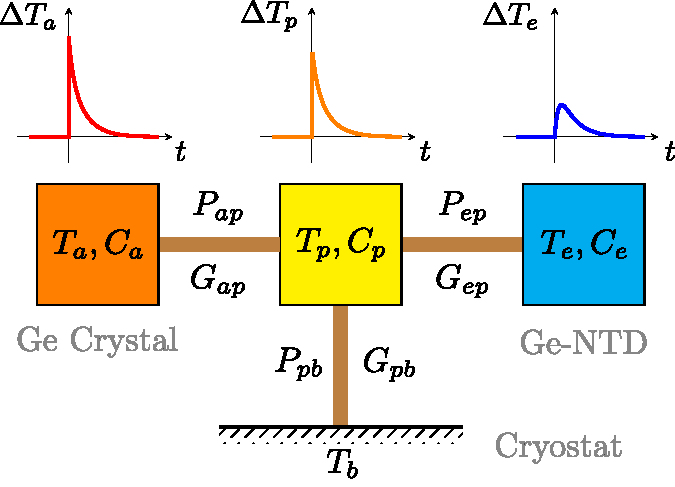
\includegraphics[scale=1]{Figures/Ethem/thermal_scheme.pdf}
\end{center}
\caption{Thermal diagram of RED1 and RED10 with representation of the diffusion of a signal created by an event in the germanium crystal on top. Each thermal bath is characterized by a temperature $T$ and a thermal capacity $C$. Each thermal link is associated with a thermal conductivity $G$ and a thermal power transfer $P$. The NTD sensor is modeled as a system of thermally coupled phonons (index $p$) and elecrons (index $e$). The absorber bath (index $a$) and the cryostat (index $b$) are both connected to the NTD phonon bath.}
\label{fig:thermal-scheme}
\end{figure}

They are connected by thermal links characterized by thermal conductivity $G$ in \si{\watt\per\kelvin}, which allows a power transfer $P$ between the baths.
At cryogenic temperatures, all heat powers are modeled using the non-linear conduction formula for non-diffusive processes \cite{Galeazzi:2003pe}.
% citation needed
The heat power from a thermal bath "1" to a thermal bath "2" is expressed as:
\begin{equation}
\label{eq:kaptiza-conduction}
P_{12} = g_{12} \left( T_2^{n_{12}} - T_1^{n_{12}}\right)
\end{equation}
with $g_{12}$ the conductance in \si{\watt\per\kelvin^{-n_{12}}} and $n_{12}$ an exponent. Both parameters depend on the interface between the thermal baths and were mainly determined experimentally.

The NTD thermistance is modeled as two separate thermal baths: the phonon bath (index $p$) and the electron bath (index $e$). Indeed at ambient temperature, the phonons and conduction electrons are in constant thermal equilibrium with the same apparent temperature $T_p = T_e$. However, at cryogenic temperature, this thermal equilibrium is reached much later and has significant impact on the thermal response of the detector. The heat power transferred from the electron bath to the phonon bath depends on their temperatures as:
\begin{equation}
\label{eq:ep-heat-power}
P_{ep}= \mathcal{V}_{NTD} g_{ep} (T_e^n - T_p^n)
\end{equation}
where $\mathcal{V}_{NTD}$ is the volume of the NTD sensor in \si{\mm^3}, $g_{ep}$ is the electron-phonon coupling constant per volume unit and $n$ is a material dependent exponent that is typically equal to 6 for thermistors such as GeNTDs.


The thermal bath associated with the absorber (index $a$) represents the phonon system of the germanium crystal. Indeed, since this material is a semiconductor at these operating temperatures, there are no free electrons in the conduction band. The absorber only exchanges heat power with the phonon system of the NTD through the thin layer of epoxy glue (with negligible thermal capacity). The heat power transferred from the absorber bath to the phonon bath is expressed as:
\begin{equation}
\label{eq:ap-heat-power}
P_{ap}=g_{glue} S_{NTD} \left( T_p^{n_g} - T_a^{n_g} \right)
\end{equation}
with $S_{NTD}$ the surface of the NTD facing the the absorber in \si{\mm^2}, $g_{glue}$ the surface thermal conductivity constant of the glue and $n_g$ an exponent. 
%These two parameters have been experimentally set in previous studies.

The thermal leakage of the detector is assured by the cabling gold wires on the gold-plated electrodes of the NTD. The heat power transferred from the phonon bath to the cryostat thermostat is:
\begin{equation}
\label{eq:pb-heat-transfer}
P_{pb}= S_{Au} g_k (T_p^{n_k} - T_b^{n_k})
\end{equation}
with $g_k$ the Kapitza conductance per unit area and the exponent $n_k=4$. The term $S_{Au}$ corresponds to the effective gold surface connecting the NTD to the copper chassis.
%two gold surfaces $S_{Au}$ (one on the NTD, one on the support) connected by gold wires. We neglect this time the thermal capacity of the surfaces and gold wires, while considering an infinite thermal capacity of the copper support, allowing to keep a fixed temperature $T_b$ at all times.

The heat channel derives the heat energy $E_{heat}$ created by a recoil in the absorber from a variation of the voltage $\Delta V$ of the NTD thermistance.
In order to maintain the proportionality between the voltage $V$ and the resistivity $R$ of the NTD in the Ohm's law \ref{eq:ohm-law}, it is polarized with a constant current $I_P$.
This is realized by adding a very high load resistance $R_L$ in series with a constant voltage source $V_B$.
The electronics schematic that allows the polarization and the measurement of the voltage at the terminals of the NTD resistor is shown in figure \ref{fig:ethem-electric-scheme}.

\begin{figure}
\begin{minipage}[c]{0.45\textwidth}
\resizebox{!}{\textwidth}{%
%\shorthandoff{:!}
\begin{circuitikz}[scale=1]
	  	\draw
	 (0.5,6) node [ground, rotate=-90] {} 
	 to [european voltage source, v=$V_B$, -*] (2,6)
	 to [european voltage source, l={\color{red} $e_{J_{RL}}$}, color=red] (2,4.5)	 
	 to [R, l_=$R_L$, -] (2,2.5)
	 to [thR, l_=$R(T_e)$, -] (2,0.5)
	 to [european voltage source, l={\color{red} $e_{J_{NTD}}$}, color=red]
	  (2,-0.5) node [ground] {}
	 (2,2.5) to [short, -o] (4,2.5) node [anchor=south] {$V$}
	 to [C, l_=$C_{cabling}$] (4,-0.5) node [ground] {} 
	 (4,2.5) to [european voltage source, l={\color{red} $e_{ampli.}$}, color=red] (6,2.5) 
	 to [ioosource, l={\color{red} $i_{ampli.}$}, color=red] (6,-0.5) node [ground] {} 
	 (6,2.5) node [anchor=south] {$U$}
	 to [short, i_={\small $i \approx 0$}, *-] (7,2.5)
	 to [amp, l=Amplifier, -] (8,2.5)
	;

\end{circuitikz}
%\shorthandon{:!}
}%
\end{minipage}
\hfill
\vrule{}
\hfill
\begin{minipage}[c]{0.45\textwidth}
\begin{center}
with simplification in the frequency-domain:
\end{center}
\resizebox{\textwidth}{!}{%
%\shorthandoff{:!}
\begin{circuitikz}
		\draw
	 (0,0) node [ground] {}
	 to [R, l_=$Z_{eq}$, -] (0,2)
	 (0,2) to [short, -o] (2,2) node [anchor=south] {$V$}
	 to [ioosource, l=$\color{red} i_{noise}$,color=red, -] 
	 (2,0) node [ground] {}
	 (2,2) to [european voltage source, l={\color{red} $e_{ampli.}$}, color=red, -] (4,2) node [anchor=south] {$U$}
	 to [short, i_={\small $i \approx 0$}, *-] (5,2)
	 to [amp, l=Amplifier, -] (6,2)
	 (0,-1.5) node [right]{$\color{red} \displaystyle i_{noise}^2=\left(\frac{e_{J_{NTD}}}{R(T_e)}\right)^2+\left(\frac{e_{J_{R_L}}}{R_L}\right)^2+i_{ampli.}^2$}
	;

\end{circuitikz}
%\shorthandon{:!}
}%
\end{minipage}
\caption{On the left, Diagram of the polarization and readout electronics. On the right, Simplified diagram in the frequency-space with the use of Thevenin-Norton transformation. The NTD resistor $R(T_e)$, the load resistor $R_L$ and the cabling capacitance $C_{cabling}$ become the equivalent complex impedance $Z_{eq}$. Noise sources appear in red. Johnson noise, $e_{J_{RL}}$ and $e_{J_{NTD}}$, and amplifier current noise $i_{ampli.}$ are grouped into a current noise $i_{noise}$ whose expression is specified.}
\label{fig:ethem-electric-scheme}
\end{figure}

On the left is the schematic of the polarization electronics with voltage and current noise sources represented in red. The capacity of the cabling $C_{cabling}$ of the electronics is taken into account. The right scheme corresponds to the simplification with multiple Thevenin-Norton transformation \cite{Mather:1982} in the context of the frequency study, which is addressed later.
A constant bias voltage $V_B$ is applied to the load resistance $R_L$, of a few \si{\giga\ohm}, in series with the NTD resistance $R(T_e)$ depending on the temperature of the electron bath $T_e$ according to the law:
\begin{equation}
R (T_e) = R_0 \exp \left( \sqrt{ \frac{T_e}{T_0} } \right)
\end{equation}
with $R_0$ and $T_0$ a characteristic resistivity and temperature of the NTD \cite{Mathimalar:2014sfa}.

The electrical system takes into account the variation of the polarization current (second-order effect as $R_L \gg R_{NTD}$).
The differential equation associated with the voltage of the NTD is:
\begin{equation}
\label{eq:electric-eq}
C_{cabling} \frac{\mathrm{d} V}{\mathrm{d} t} = \frac{V_B - V}{R_L} - \frac{V}{R(T_e)}
\end{equation}

Due to the polarization of the NTD, a Joule effect is present, coupling the electron thermal bath and the electronics:
\begin{equation}
\label{eq:joule-ntd}
P_J= I_P^2 \cdot R(T_e)= \frac{V^2}{R(T_e)}
\end{equation}

The heat equations associated with each thermal bath is derived from all the previously defined heat powers. 
The thermal equation for the electron bath is obtained from the NTD Joule heating (eq. \ref{eq:joule-ntd}) and the thermal coupling to the phonon bath (eq. \ref{eq:ep-heat-power}) such that:
\begin{equation}
\label{eq:heat-eq-electron}
 C_e \frac{\mathrm{d} T_e}{\mathrm{d} t} = \frac{V^2}{R(T_e)} - \mathcal{V}_{NTD} g_{ep} \left( T_e^{n} - T_p^{n} \right)
\end{equation}

For the NTD phonon system, we have the power from the phonon-electron coupling $P_{ep}$, the power transfer with the absorber (eq. \ref{eq:ap-heat-power}), and the thermal leakage (eq. \ref{eq:pb-heat-transfer}) to the cryostat. This phonon bath is described by the heat equation:
\begin{equation}
\label{eq:heat-eq-phonon}
C_p \frac{\mathrm{d} T_p}{\mathrm{d} t}
=
-g_{glue} S_{NTD} \left( T_p^{n_g} - T_a^{n_g} \right) 
+ V_{NTD} g_{ep} \left( T_e^{n} - T_p^{n} \right)
- g_k S_{Au} \left( T_p^{n_k} - T_b^{n_k} \right)
\end{equation}

The thermal equation for the absorber bath is simply derived from the heat conduction through the glue (eq. \ref{eq:ap-heat-power}):
\begin{equation}
\label{eq:heat-eq-absorber}
C_a \frac{\mathrm{d} T_a}{\mathrm{d} t} = g_{glue} S_{NTD} \left( T_p^{n_g} - T_a^{n_g} \right)
\end{equation}

By bringing together the three heat equations \ref{eq:heat-eq-absorber}, \ref{eq:heat-eq-electron} and \ref{eq:heat-eq-phonon} as well as the differential equation \ref{eq:electric-eq} associated with the polarization electronics, we can compose a system of coupled differential equations that completely describes the electro-thermal model of the detector RED10 schematized in the figures \ref{fig:thermal-scheme} and \ref{fig:ethem-electric-scheme}:

\begin{equation}
\begin{cases}
\label{eq:ethem-system}
\displaystyle C_a \frac{\mathrm{d} T_a}{\mathrm{d} t} &= g_{glue} S_{NTD} \left( T_p^{n_g} - T_a^{n_g} \right) \\[10pt]
\displaystyle C_p \frac{\mathrm{d} T_p}{\mathrm{d} t}
&=
-g_{glue} S_{NTD} \left( T_p^{n_g} - T_a^{n_g} \right) 
+ \mathcal{V}_{NTD} g_{ep} \left( T_e^{n} - T_p^{n} \right)
- g_k S_{Au} \left( T_p^{n_k} - T_b^{n_k} \right) \\[10pt]
\displaystyle C_e \frac{\mathrm{d} T_e}{\mathrm{d} t} &= \frac{V^2}{R(T_e)} - \mathcal{V}_{NTD} g_{ep} \left( T_e^{n} - T_p^{n} \right) \\[10pt]
\displaystyle C_{cabling} \frac{\mathrm{d} V}{\mathrm{d} t} &= \frac{V_B - V}{R_L} - \frac{V}{R(T_e)}
 \end{cases}
\end{equation}


\subsection{Steady State Solution}
\label{par:stationnary-state}
\label{par:steady-state}

The study of the steady state allows to obtain the physical quantities around which the disturbances of the system will occur. It is essential to calculate it in order to obtain the values of the NTD resistance, thermal capacities and thermal conductivities. It is also necessary to perform a linearization step afterwards. The steady state is experimentally defined by the cryostat temperature $T_b$ and the bias voltage $V_B$. 

It is sufficient to cancel the time derivative terms in the system of equations \ref{eq:ethem-system} to obtain the system of equations in the stationary state with ($\bar{T}_a, \bar{T}_p, \bar{T}_e, \bar{V}$) being the solutions of the stationary state:
\begin{equation}
\begin{cases}
\label{eq:ethem-system-stationnary}
0 &= g_{glue} S_{NTD} \left( \bar{T}_p^{n_g} - \bar{T}_a^{n_g} \right)  \\[8pt]
0 &= -g_{glue} S_{NTD} \left( \bar{T}_p^{n_g} - \bar{T}_a^{n_g} \right) + \mathcal{V}_{NTD}  g_{ep} \left( \bar{T}_e^{n} - \bar{T}_p^{n} \right) - g_k S_{Au} \left( \bar{T}_p^{n_k} - \bar{T}_b^{n_k} \right)  \\[8pt]
0 &= \frac{V^2}{R(\bar{T}_e)} - \mathcal{V}_{NTD} g_{ep} \left( \bar{T}_e^{n} - \bar{T}_p^{n} \right)  \\[8pt]
0 &= \frac{V_B - V}{R_L} - \frac{V}{R(\bar{T}_e)}
 \end{cases}
\end{equation}

These algebraic equations are non-linear due to the expressions of the heat power (eq. \ref{eq:kaptiza-conduction}) and of the NTD resistance \ref{eq:ntd-resistivity}. It is therefore necessary to use a numerical resolution to solve this system. 


\subsection{Response in the Time Domain}
\label{par:time-domain}

Solving the system of equations \ref{eq:ethem-system} would give the exact expressions of the temporal evolution of the temperatures of the different baths $T_a(t), T_p(t), T_e(t)$ and of the voltage at the terminals of the NTD $V(t)$.
However, the very strong non-linearity of the system does not allow an analytical resolution.
Nevertheless, only the response of the system to an event is of interest. As reference, a particle depositing a heat energy of \SI{1}{\kilo\eV} in the absorber induces a temperature increase of the order of $\mathcal{O}(100)\ \si{\micro\kelvin}$, which in turn, gives a voltage variation at the terminals of the NTD of the order of $\mathcal{O}(100)\ \si{\nano\volt}$. 
It is thus a question of studying the response of the system to small signals. We propose to apply a first-order perturbation theory \cite{Pyle:2015pya} to the system of equations \ref{eq:ethem-system} with:
\begin{equation}
\label{eq:linearization}
\begin{cases}
T_a(t) &\simeq \bar{T}_a + \Delta T_a (t) \\
T_p(t) &\simeq \bar{T}_p + \Delta T_p (t) \\
T_e(t) &\simeq \bar{T}_e + \Delta T_e (t) \\
V(t) &\simeq \bar{V} + \Delta V (t) \\
\end{cases}
\end{equation}
With this linearization of the physical quantities, it is possible to define thermal conductivities $G$ for the different thermal links :
\begin{itemize}
\item glue crystal-NTD: \begin{equation}\label{eq:g1} G_{ap}^a  = n_g g_{glue} S_{NTD} \bar{T}_a^{n_g-1} \qquad \textrm{and} \qquad G_{ap}^p  = n_g g_{glue} S_{NTD} \bar{T}_p^{n_g-1}
\end{equation}
\item electrons-phonon coupling: \begin{equation}\label{eq:g2} G_{ep}^e  = n g_{ep} \mathcal{V}_{NTD} \bar{T}_e^{n-1} \qquad \textrm{and} \qquad G_{ep}^p  = n g_{ep} \mathcal{V}_{NTD} \bar{T}_p^{n-1}
\end{equation}
\item thermal leakage through gold wires: \begin{equation}\label{eq:g3} G_{pb} = n_k g_{k} S_{Au} \bar{T}_p^{n_k-1}
\end{equation}
\end{itemize}
%Note that the conductivities have a "direction" of use as they depend on the temperature of the baths.
 By subtracting the steady state equation \ref{eq:ethem-system-stationnary} from the original system \ref{eq:ethem-system}, we then obtain a system of coupled linear equations:
\begin{equation}
\label{eq:ethem-system-temp}
\begin{cases}
\displaystyle C_a \frac{d \Delta T_a}{d t}
	&= -G_{ap}^a \Delta T_a + G_{ap}^p \Delta T_p 
	 \\[10pt]
\displaystyle C_p \frac{d \Delta T_p}{d t} 
	&= +G_{ap}^a \Delta T_a - G_{ap}^p \Delta T_p
	+ G_{ep}^e \Delta T_e - G_{ep}^p \Delta T_p
	- G_{pb}^p \Delta T_p
	 \\[10pt]
\displaystyle C_e \frac{d \Delta T_e}{d t}
	&= - G_{ep}^e \Delta T_e + G_{ep}^p \Delta T_p
	+2\frac{\bar{V}}{R(\bar{T}_e)} \Delta V - \frac{\bar{V}^2}{R(\bar{T}_e)^2} \left.\frac{d R}{d T}\right\vert_{T_e} \Delta T_e
 	 \\[10pt]
\displaystyle C_{cabling} \frac{d \Delta V}{d t} &= - \left( \frac{1}{R_L} + \frac{1}{R(\bar{T}_e)} \right) \Delta V + \frac{\bar{V}}{R(\bar{T}_e)^2} \left.\frac{d R}{d T}\right\vert_{\bar{T}_e} \Delta T_e
\end{cases}
\end{equation}
This can be simplified to:
\begin{equation}
\label{eq:ethem-system-temp-simplified}
\begin{cases}
\displaystyle \frac{d \Delta T_a}{d t}
	&= -\frac{G_{ap}^a}{C_a} \Delta T_a + \frac{G_{ap}^p}{C_a} \Delta T_p 
	 \\[10pt]
\displaystyle \frac{d \Delta T_p}{d t} 
	&= \frac{G_{ap}^a}{C_p} \Delta T_a - \frac{G_{ap}^p+G_{ep}^p+G_{pb}^p}{C_p} \Delta T_p	+ \displaystyle \frac{G_{ep}^e }{C_p}\Delta T_e
	 \\[10pt]
\displaystyle \frac{d \Delta T_e}{d t}
	&= \frac{G_{ep}^p}{C_e} \Delta T_p - \frac{1}{C_e} \left(G_{ep}^e + \frac{\bar{V}^2}{R(\bar{T}_e)^2} \left.\frac{d R}{d T}\right\vert_{\bar{T}_e}\right) \Delta T_e 
	+2 \frac{1}{C_e} \frac{\bar{V}}{R(\bar{T}_e)} \Delta V
 	 \\[10pt]
\displaystyle \frac{d \Delta V}{d t} &= \frac{1}{C_{cabling}} \frac{\bar{V}}{R(\bar{T}_e)^2} \left.\frac{d R}{d T}\right\vert_{\bar{T}_e} \Delta T_e - \frac{1}{C_{cabling}}\left( \frac{1}{R_L} + \frac{1}{R(\bar{T}_e)} \right) \Delta V
\end{cases}
\end{equation}

A system of linear equations is now being studied. It is thus possible to solve them analytically. For this purpose, this system of equations can be rewritten in matrix form to facilitate the calculations. The vector $\bm{\phi}$ containing the temperature and voltage perturbations is introduced:
\begin{equation}
\label{eq:ethem-phi}
\bm{\phi} = 
\left( \begin{array}{c}
\Delta T_a\\
\Delta T_p\\
\Delta T_e\\
\Delta V
\end{array} \right)
\end{equation}
The simplified system of equation \ref{eq:ethem-system-temp-simplified} is now simply expressed as the matrix equation:
\begin{equation}
\label{eq:ethem-matrix-eq}
\frac{d \bm{\phi}}{d t}= - \bm{M} \bm{\phi} + \bm{F}(t-t_0)
\end{equation}
where $\bm{M}$ is the matrix regrouping the electro-thermal coupling terms. It is directly derived from the previous equations \ref{eq:ethem-system-temp-simplified}, and is expressed as:
\begin{equation}
\label{eq:ethem-coupling-mat}
\bm{M} = 
\left( \begin{array}{cccc}
 \frac{G_{ap}^a}{C_a}&-\frac{G_{ap}^p}{C_a}&0&0 \\
 -\frac{G_{ap}^a}{C_p}&\frac{G_{ap}^p+G_{ep}^p+G_{pb}^p}{C_p}&-\frac{G_{ep}^e}{C_p}&0 \\
0&-\frac{G_{ep}^p}{C_e}&\frac{1}{C_e}\left(G_{ep}^e + \frac{\bar{V}^2}{R(T_e)^2}  \left.\frac{d R}{d T}\right\vert_{\bar{T}_e} \right)&-\frac{2}{C_e}\frac{\bar{V}}{R(T_e)}\\
0&0&-\frac{1}{C_{cabling}}\frac{\bar{V}}{R(T_e)^2} \left.\frac{d R}{d T}\right\vert_{\bar{T}_e} &\frac{1}{C_{cabling}}\left( \frac{1}{R_L} + \frac{1}{R(T_e)} \right)
\end{array} \right)
\end{equation}
A source term $\bm{F}$ has also been added to contain the energy perturbation in the detector and the various sources of interference noise. In the case of a particle depositing a heat energy $E$ in the absorber, this term is expressed as,
\begin{equation}
\bm{F}(t-t_0) = 
\left( \begin{array}{c}
E/C_a \\
0 \\
0 \\
0
\end{array} \right) \delta (t-t_0)
\end{equation}
The deposition of the recoil energy, the relaxation of the phonons created in the absorber, and the temperature rise of the absorber are considered instantaneous processes, hence the use of the Dirac function $\delta (t-t_0)$. A variant of this model consists in assigning a relaxation time to the phonons and taking into account the temperature rise of the thermal baths during phonon relaxation.

The general solution of the equation \ref{eq:ethem-coupling-mat} is a linear combination of $N$ exponential, with $N=4$ corresponding to the dimensions of the system, each characterized by a time constant. Their expressions are obtained by diagonalizing the coupling matrix $\bm{M}$, which shifts the framework to the basis formed by the eigenvectors of the system solutions. We consider, for $i \in \{1,2,3,4\}$, the eigenvectors $\bm{v}_i$ and the associated eigenvalues $f_i(t)$ to write these solutions:
\begin{equation}
\label{eq:eigen-solution}
\bm{f}_i(t) = f_i(t) \bm{v}_i
\end{equation}
Without considering the source term, we introduce these expressions into the matrix equation \ref{eq:ethem-matrix-eq} to give
\begin{equation}
\label{eq:eigen-solution-ode}
\frac{d \bm{f}_i(t)}{d t} = -f_i(t) \bm{M} \bm{v}_i = -\lambda_i f_i(t) \bm{v}_i
\end{equation}
Solving this equation leads to the expression of the solutions in the basis of the eigenvectors:
\begin{equation}
f_i(t) = A_i e^{-t/\tau_i} \bm{v}_i
\end{equation}
with $A_i$ the normalization constant and $\tau_i=1/\lambda_i$ the characteristic time constant of the solution. The general solution of \ref{eq:ethem-coupling-mat} is then expressed in the new basis as
\begin{equation}
\label{eq:eigein-solution-expr}
\bm{f}(t) = \sum_i A_i e^{-t/\tau_i} \bm{v}_i
\end{equation}
To make the link between the basis of the eigenvectors and the temperature and voltage fluctuations, the $\bm{f}$ solution must be projected onto the 4 orthogonal vectors forming the vector $\bm{\phi}$ such that :
\begin{equation}
\label{eq:gen-solution}
\phi_j = \bm{f} \cdot \bm{\phi}_j = \sum_i^4 f_i(t) \bm{v}_i \cdot \bm{\phi}_j = \sum_i P_{ij} f_i(t) = \sum_i P_{ij} A_i e^{-t/\tau_i}
\end{equation}
where $P_{ij}$ designates the vectors composing the transfer matrix satisfying $\bm{M}=\bm{P} \bm{D} \bm{P}^{-1}$.

To set the normalization constants $A_i$, the initial conditions of the system are considered:
\begin{equation}
\bm{\phi}(0) = \bm{F}(0) =
\left( \begin{array}{c}
\sum_i P_{ai} A_i\\
\sum_i P_{pi} A_i\\
\sum_i P_{ei} A_i\\
\sum_i P_{vi} A_i
\end{array} \right) = \bm{P} \bm{A}
\qquad \longrightarrow \qquad \bm{A}=\bm{P}^{-1} \bm{\phi} (0)
\label{eq:ethem-initial-value}
\end{equation}
with $\bm{A}$ the vector containing the constants $A_i$.

The study of a detector in time is equivalent to solving the matrix equation \ref{eq:ethem-coupling-mat} and thus to find the eigenvalues and eigenvectors of the coupling matrix $\bm{M}$. The electro-thermal model is now completely described in the time domain.


\subsection{Response in Frequency Domain}
\label{par:ethem-frequency-domain}

The study of noise leading to the calculation of the resolution of the detector requires to describe now the behavior in frequency domain. Indeed, the noises of a system are characterized from their power spectral densities (PSD).
We consider the Fourier transform of the matrix equation \ref{eq:ethem-matrix-eq}:
\begin{equation}
\bm{C} (i\omega + \bm{M})  \bm{\tilde{\phi}}  (\omega) = \bm{Z} (\omega) \bm{\tilde{\phi}} (\omega)  = \bm{C} \bm{\tilde{F}} (\omega) \qquad \textrm{with} \qquad \bm{C} = \left( \begin{array}{cccc}
 C_a&0&0&0 \\
0&C_p&0&0\\
0&0&C_e&0\\
0&0&0&C_{cabling}
\end{array} \right)
\end{equation}
where we introduce the matrix $\bm{Z}$ containing the electro-thermal coupling terms expressed in the Fourier space. The equation is rewritten by explaining the terms of the matrices and vectors: 
\begin{equation}
\label{z-mat}
\bm{Z} (\omega) \bm{\tilde{\phi}} (\omega) =
\left( \begin{array}{cccc}
 \frac{1}{a}&-g&0&0 \\
-b&\frac{1}{c}&-h&0\\
0&-d&\frac{1}{e}-k&-l\\
0&0&-f&Z_{eq}^{-1}
\end{array} \right)
\left( \begin{array}{c}
\Delta T_a\\
\Delta T_p\\
\Delta T_e\\
\Delta V
\end{array} \right)
 =
\left( \begin{array}{c}
W\begingroup\color{red} - P_{ap}\endgroup\\
\begingroup\color{red}  P_{ap} + P_{ep} + P_{bp}\endgroup\\
\begingroup\color{red} - P_{ep}\endgroup\\
\begingroup\color{red}  i_{noise} \endgroup
\end{array} \right)
=  \bm{C} \bm{\tilde{F}} (\omega)
\end{equation}
The terms of the vector $\bm{C} \bm{\tilde{F}} (\omega)$ corresponds to the perturbation sources in the form of heat power or current source. The heat power $W$ comes from the recoil induced by an interacting particle.
% Noise power
All the red terms corresponds to the various noise sources affecting the detector performance. The heat powers $P_{xy}$ with $x,y \in \{ a,p,e,b \}$ are generated by the thermodynamic fluctuation noise (TFN) at the interface between two thermal baths. The current source $i_{noise}$ corresponds to the propagation of all the electronics noise sources propagated to the terminals of the NTD.

The coefficients of the matrix $\bm{Z}$ are derived from the system of linearized equations \ref{eq:ethem-system-temp-simplified} such as :
\begin{equation}
\begin{aligned}[c]
a &=(i C_a \omega + G_{ap}^a)^{-1} \\
b &=G_{ap}^a \\
c &=(i C_p \omega + G_{ap}^p + G_{ep}^p + G_{pb})^{-1} \\
d &=G_{ep}^p \\
e &=(i C_e \omega + G_{ep}^e)^{-1}\\
f &=\frac{(dR/dT) V}{R^2} 
\end{aligned}
\qquad \qquad
\begin{aligned}[c]
g &=G_{ap}^p \\
h &=G_{ep}^e \\
k &=- \frac{(dR/dT) V^{2}}{R^{2}} \\
\ell &=\frac{2 V}{R}
\end{aligned}
\label{coef}
\end{equation}
and with the complex impedance $Z_{eq}$, containing the electrical components of the bias circuit according to the figure \ref{fig:ethem-electric-scheme}, expressed as:
\begin{equation}
Z_{eq} = \left(\frac{1}{R_L} + \frac{1}{R(T_e)} + i\omega C_{cabling}\right)^{-1}
\end{equation}
The expression of the vector of fluctuations $\bm{\phi}$ is obtained by inverting the coupling matrix $\bm{Z}$ as,:
\begin{equation}
\bm{\tilde{\phi}} (\omega) =
\left( \begin{array}{c}
\Delta \tilde{T}_a\\
\Delta \tilde{T}_p\\
\Delta \tilde{T}_e\\
\Delta \tilde{V}
\end{array} \right)
=
\left( \begin{array}{cccc}
 Z_{aa}^{-1}&Z_{ap}^{-1}&Z_{ae}^{-1}&Z_{av}^{-1} \\
 Z_{pa}^{-1}&Z_{pp}^{-1}&Z_{pe}^{-1}&Z_{pv}^{-1}\\
 Z_{ea}^{-1}&Z_{ep}^{-1}&Z_{ee}^{-1}&Z_{ev}^{-1}\\
 Z_{va}^{-1}&Z_{vp}^{-1}&Z_{ve}^{-1}&Z_{vv}^{-1}
\end{array} \right)
\left( \begin{array}{c}
\Delta \tilde{P}_a\\
\Delta \tilde{P}_p\\
\Delta \tilde{P}_e\\
\Delta \tilde{I}
\end{array} \right)
= \bm{Z}^{-1}(\omega) \bm{\tilde{F}} (\omega)
\end{equation}
We note here that the matrix formalism coupled with a numerical calculation tool allows an easy access to the temperature and voltage perturbations from the coupling matrix $\bm{M}$ and external power sources contained in the $\bm{\tilde{F}}(w)$ vector.

% Block diagram
In spite of this simplification of the calculations, the understanding of the couplings between the different physical quantities is not so easy. A better understanding is possible by converting the system of equations \ref{eq:ethem-coupling-mat} into a block diagram formalism. 
An illustration of the matrix equation is displayed in figure \ref{fig:block-diagram} as a block diagram. This representation is useful to understand the localization of the different signal-induced or noise-induced perturbations in the electro-thermal system. We find there the coupling coefficients used in the coupling matrix $\bm{Z}$ as well as the external power sources. It is easier to visualize the coupling between the different baths as well as the diffusion of the power deposited by a particle in the absorber $W$.

\begin{figure}
\begin{center}
\resizebox{\textwidth}{!}{%
\begin{tikzpicture}
	    \sbEntree{W}
    \sbCompSum{C1}{W}{-}{+}{+}{}
    	\sbRelier{W}{C1}
        \sbNomLien[0.8]{W}{$W$}
    \sbBloc{a}{$a$}{C1}
        \sbRelier{C1}{a}
    \sbBloc[3]{b}{$b$}{a}
        \sbRelier[$\Delta T_a$]{a}{b}  
    \sbCompSum{C2}{b}{+}{+}{+}{}
        \sbRelier{b}{C2}      
    \sbBlocL{c}{$c$}{C2}
    \sbBloc[3]{d}{$d$}{c}
    	\sbRelier[$\Delta T_p$]{c}{d}
    \sbCompSum{C3}{d}{-}{+}{+}{}
    	\sbRelier{d}{C3}		
    \sbBlocL{e}{$e$}{C3}	      
    \sbBloc[3]{f}{$f$}{e}
    	\sbRelier[$\Delta T_e$]{e}{f}
    \sbCompSum{C4}{f}{+}{}{+}{}
        \sbRelier{f}{C4}
    \sbBlocL{Z}{$Z_{eq}$}{C4}
    \sbCompSum[5]{C5}{Z}{+}{}{+}{}
        \sbRelier[$\Delta V$]{Z}{C5}
    \sbSortie{V}{C5}
        \sbRelier{C5}{V}
        \sbNomLien[0.8]{V}{$\Delta U$}
    
    \sbDecaleNoeudy[5]{a-b}{down1}
	\sbBlocr{g}{$g$}{down1}
		\sbRelieryx{c-d}{g}
    	\sbRelierxy{g}{C1}
    \sbDecaleNoeudy[8]{c-d}{down2}
	\sbBlocr{h}{$h$}{down2}
		\sbRelieryx{e-f}{h}
    	\sbRelierxy{h}{C2}
	\sbDecaleNoeudy[10]{d}{down5}
	\sbCompSum{C6}{down5}{}{+}{}{+}
	\sbBloc{k}{$k$}{C6}
	\sbDecaleNoeudy[13]{C4-Z}{down4}
	\sbBlocr{l}{$\ell$}{down4}
		\sbRelier[$\Delta P_J$]{C6}{C3}
		\sbRelieryx{e-f}{k}
    	\sbRelier{k}{C6}	
		\sbRelieryx{Z-C5}{l}
    	\sbRelierxy{l}{C6}
    
    \sbStyleLien{red,text=red}
    \sbDecaleNoeudy[-4]{C1}{Pap}
    	\sbRelier{Pap}{C1}
    	\sbNomLienCustom[0.3]{Pap}{$P_{ap}$}
    \sbDecaleNoeudy[-4]{C2}{sumP}
    	\sbRelier{sumP}{C2}
    	\sbNomLienCustom[0.3]{sumP}{$P_{ap}+P_{ep}+P_{bp}$}
    \sbDecaleNoeudy[-4]{C3}{Pep}
    	\sbRelier{Pep}{C3}
    	\sbNomLienCustom[0.3]{Pep}{$P_{ep}$}
    \sbDecaleNoeudy[-4]{C4}{i}
    	\sbRelier{i}{C4}
    	\sbNomLienCustom[0.3]{i}{$i_{noise}$}  
    \sbDecaleNoeudy[-3]{C5}{eA}
    	\sbRelier{eA}{C5}
    	\sbNomLienCustom[0.3]{eA}{$e_{ampli.}$}   

\end{tikzpicture}
}%
\end{center}
\caption{Block diagram of the electro-thermal model with the power injection of an event $W$, power noise $P_{ap}, P_{ep}, P_{pb}$, current noise $i_{noise}$ and voltage noise $e_{ampli.}$. The block coefficients are specified in (\ref{coef}). Block diagram formalism and matrix formalism are equivalent and result in identical expressions for sensitivity and noise calculations.
}
\label{fig:block-diagram}
\end{figure}

By reading the block diagram from left to right, we can follow the propagation of the signal in the detector and the different feedback mechanisms between each node. The power $W$ is injected in the absorber bath from the heat energy $E_{heat}$ released by a recoil. This bath is also affected with the TFN heat power $-P_{ap}$, associated with its thermal link with the NTD phonon bath, and the heat transfer $g \Delta T_p$ coming from the NTD phonon bath. The term $a$ converts all the heat powers incoming in the absorber bath (first node on the block diagram) into the temperature fluctuation $\Delta T_a$. The latter is in turn converted back with the term $b$ into a heat power incoming on the NTD phonon bath (second node of the block diagram). The subsequent propagation of the signal and noises in the system eventually reaches the end node on the right of the block diagram corresponding to the measured voltage signal $\Delta U$ amplified by the electronics (see the circuit scheme \ref{fig:ethem-electric-scheme} for reference).

% This bath is affected by the TFN noises of all its thermal links $P_{ap}$, $P_{ep}$ and $P_{pb}$

The response of the system to an event is characterized by the sensitivity $s_V$. In the case of a particle interaction depositing all the recoil energy in the absorber, the sensitivity is expressed as ${s}_V(\omega) = Z_{va}^{-1}\hat{p}(\omega)$ with $\hat{p}(\omega)$ the Fourier transform of the signal into power $W$. The approximation of an instantaneous recoil energy deposit gives $\hat{p}(\omega) = \hat{\delta} = 1$, which tremendously simplifies the calculations.
The variant where we consider the phonon relaxation time requires to multiply by the low-pass function $\hat{p}(\omega) = 1/(1+i\omega \tau_P)$ with $\tau_P$ the time constant corresponding to the phonon relaxation time within the detector.
Other direct detection experiments, such as CDMS \cite{Billard:2012}, work by detecting athermal phonons that can transfer between the different components of the detector before relaxing. Thus, it is possible to have a fraction $\epsilon$ of the phonons, produced during an event, leaving the absorber to the NTD and relax there. We would then observe a temperature rise directly in the NTD sensor, in addition to the temperature rise in the absorber. Taking this possibility into account, the sensitivity of the system is rewritten:
\begin{equation}
\label{sv}
\hat{s}_V(\omega) = \left[(1-\epsilon) Z_{va}^{-1} + \epsilon Z_{ve}^{-1}\right]\hat{p}(\omega) \qquad [V/W]
\end{equation}
The $\epsilon$ fraction of so-called "athermal" phonons depends very strongly on the geometry of the germanium crystal, its polishing, the glue used between the absorber and the NTD, and surely other parameters of the experiment that are not yet identified. The presence of athermal phonons is detected thanks to the signal shape: the temperature rise of the NTD is faster and an exponential contribution appears characterized by the time constant $\tau_P$. We will see later in this chapter that the RED10 detector has a relatively large fraction of athermal phonons which is estimated by the signal shape.

The resolution of the block-diagram \ref{fig:block-diagram} ensures that the feedback loop associated with the Joule power $\Delta P_J$ is negative,
%\begin{equation}
%\Delta P_J 
%= k \cdot \Delta T_e + \ell \cdot \Delta V
%= -\frac{(dR/dT) V^{2}}{R^{2}} \Delta T_e + 2 \frac{V}{R} \Delta V
%= \frac{V}{R} \left( 2 \Delta V - \frac{dR}{dT} \Delta T_e \frac{V}{R} \right)
%\end{equation}
 allowing the stability of the NTD resistor polarization.
Indeed, the temperature rise $\Delta T_e$ created by the bias current in the NTD decreases its resistance $R$ due to its resistivity characteristic (eq. \ref{eq:ntd-resistivity}) being monotically decreasing. This, in turn, reduces the Joule effect $P_J \propto R$ assuming the bias current $I_P$ being almost constant.
This negative feedback is characteristic from the thermal sensor technology used: the resistance of the NTDs decreases with temperature. The other main thermal sensor technology used in cryogenic bolometers, the Transition Edge Sensors (TES) based on the superconductive transition of a material have 
an increasing resistance with the temperature \cite{Billard:2012} \cite{Figueroa:2006}. In this situation, this would result in a positive feedback which would eventually lead to the thermal sensor heating itself out of its sensitivity range. To obtain negative feedback and polarization stability, these experiments use voltage polarization and not current polarization. Indeed, we are in the case $P_J=V^2/R$ with $V$ kept constant.

Another advantage of this negative feedback is the attenuation of some disturbances: we can then reduce the impact of noise in general and in particular thermal noises \cite{Mather:1982}. 
The thermal noises are the intrinsic limiting phenomenon interfering with the measurement. Generally speaking, the only way to reduce them is to lower the temperature of the cryostat further, which is difficult because we then come up against the limit of cryogenic technology.

It is now possible to access the noise spectral density referred to the voltage at the terminals of the NTD by quadratically summing the different noise sources, considering that they are not correlated with each other. The total noise power spectral density is expressed in \si{\volt^2\per\Hz} as,
\begin{equation}
\label{eq:ethem-psd-total}
S_{V,total} = \sum_i^{sources} \left\vert \sum_j^{a,p,e,v} Z_{v,j}^{-1} (\omega) \tilde{F}_j(\omega) \right\vert^2
\end{equation}
where the quadratic summation is performed on all noise sources, and the $v$ index refers to the coefficients of the inverted coupling matrix relative to the voltage across the NTD.

The different noise sources and the level at which they occur are shown in red on the figure \ref{fig:block-diagram}. First of all we have the presence of TFN heat power presents for each thermal link in the system: $P_{ap}, P_{pb}, P_{ep}$. The PSD of these power fluctuations in the link connecting a bath at $T_i$ and a bath at $T_j$ is expressed in \si{\watt^2\per\Hz} as
\cite{Juillard:1999} \cite{Ashcroft:1976} :
\begin{equation}
S_{P,ij} = 2k_B(T_i^2 + T_j^2) G_{ij}
\end{equation}
with the thermal conductivity of the link $G_{ij}$.
Thanks to the perturbation theory, we have obtained expressions of the conductivities (eq. \ref{eq:g1},\ref{eq:g2} and \ref{eq:g3}) depending on the direction of heat transfer considered. Since the behavior of TFN noise with such conductivities is not properly defined, an effective thermal conductivity for TFN noise is approximated as the average of these two conductivities relative to the thermal link. Since TFN noise is associated with a thermal bond, it affects two thermal baths. In order to respect the principle of energy conservation, the anti-correlation of the contributions of a TFN noise in the two baths must be taken into account. By adapting the equation \ref{eq:ethem-psd-total}, one can obtain an intermediate PSD in \si{\volt^2\per\Hz} that includes all the TFN noise terms:
\begin{multline}
S_{V,TFN} = 2k_B \times  \left[ (T_a^2 + T_p^2) G_{ap} \left\vert Z_{vp}^{-1} - Z_{va}^{-1} \right\vert^2 \right. \\ \left. + (T_e^2 + T_p^2) G_{ep} \left\vert Z_{vp}^{-1} - Z_{ve}^{-1} \right\vert^2 + (T_p^2 + T_b^2) G_{pb} \left\vert Z_{vp}^{-1}\right\vert^2 \right]
\end{multline}
Following the noises indicated on the block diagram \ref{fig:block-diagram}, we now have the intervention of a current noise $i_{noise}$ which comes from the Thevenin-Norton transformation of the electric circuit presented on the figure \ref{fig:ethem-electric-scheme}. It corresponds to the quadratic sum of the Johnson noises $e_{J_{R_L}}, e_{J_{NTD}}$ related to the load and NTD resistors and the current noise introduced by the amplification electronics $i_{ampli.}$ which is expressed in \si{\ampere^2\per\Hz} as: 
\begin{equation}
\label{i-bruit}
i_{noise}^2 = i_{ampli}^2 + \left( \frac{e_{J_{R_L}}}{R_L} \right)^2 + \left( \frac{e_{J_{NTD}}}{R(T_e)} \right)^2
\end{equation}
An electrical resistance of value $R$ at temperature $T$ has its terminal voltage fluctuating randomly due to the Johnson noise whose PSD is expressed in \si{\volt^2\per\Hz}:
\begin{equation}
e_{J_R}^2 = 4k_B T R
\end{equation}
This gives the contribution of the Johnson noises to the total noise PSD:
\begin{align}
S_{V,R(T_e)} &= \frac{4 k_B T_e R(T_e)}{R(T_e)^2} \left\vert Z_{vv}^{-1}\right\vert^2
\\
S_{V,R_L} &= \frac{4 k_B T_{R_L} R_L}{R_L^2} \left\vert Z_{vv}^{-1}\right\vert^2
\end{align}
The contribution of the Johnson noise is weighted by the corresponding resistance, which is ultimately a voltage divider. Thus, the voltage fluctuations at the terminals of the load resistor $R_L$ are 2 to 3 orders higher than the voltage fluctuations at the terminals of the NTD sensor $R(T_e)$ but the division by $R_L$ allows the Johnson noise of the NTD to dominate in the calculation.

The last two current noise terms $i_{ampli}$ and $e_{ampli}$ come from the amplification electronics simply represented by an amplifier follower on the figure \ref{fig:ethem-electric-scheme}. They are dependent on the type of electronics used and must be determined experimentally. Their contribution to the total PSD is expressed in \si{\volt^2\per\Hz} as :
\begin{align}
\label{eq:ethem-noise-ampli}
S_{V,i_{ampli.}} &= i_{ampli.}^2 \left\vert Z_{vv}^{-1}\right\vert^2
\\
S_{V,e_{ampli.}} &= e_{ampli.}^2
\end{align}
Indeed, there is no current leakage to the amplifier electronics, so the amplifier voltage noise term $e_{ampli.}$ affects the measurement independently of the upstream circuit.

Now that we have expressed the spectral noise density on the measured voltage and the sensitivity of the system to the signal, it is possible to perform the calculation of the detector resolution. To do this, we introduce the Noise-Equivalent Power (NEP). This value corresponds to the PSD of the noise produced in the absorber (and the electron system, if athermal phonons are considered) which would induce a voltage noise PSD identical to the total noise PSD already calculated by the formula \ref{eq:ethem-psd-total}. In a simpler way, it is a "tool" to compare the sensitivity of the system and the spectral density of noise affecting the measurement, independently of the signal and noise sources. In this system with the signal being a power, the NEP is expressed in \si{\watt\per\sqrthz}. Its expression is given by the formula:
\begin{equation}
\label{eq:nep}
NEP^2(\omega) =  \frac{S_{V,total}}{|\hat{s}_V|^2}
\end{equation}
The NEP can be interpreted as the inverse of the signal-to-noise ratio, taking into account the system bandwidth. It can therefore be expected that the energy resolution $\sigma_E$ of the detector will be related to this value. Calculations described in \cite{Enss:2005md} gives the expression of the energy resolution in Joules as a function of the NEP:

\begin{equation}
\label{eq:resolution}
\displaystyle{ \sigma_E^2 = \left( \int_{0}^{\infty} \frac{\mathrm{d}\omega}{2\pi}\frac{4}{|NEP(\omega)|^2}\right)^{-1} } \qquad [J^2]
\end{equation}
The integration on the pulsation $\omega$ from $0$ to infinity is only theoretical. Experimentally, these integration bounds are limited by the duration of the measurement, which sets the lower bound, and the Nyquist frequency, which sets the upper bound. 
Considering the recoil energy range associated with the recoils in a cryogenic detectors, it is customary to reason in \si{eV} and therefore to multiply the resolution by the conversion factor $u=(1.602\times 10^{-19})^{-1} = \SI{6.241e18}{\eV\per\joule}$.


\section{Application of the Model to Experimental Data}

In the previous section, we have set up the electro-thermal model of a RED detector with a single thermal sensor, like RED1 and RED10. Thus this model can now be applied to characterize the noise affecting the measurement of the heat channel as well as to the characterization of the RED10 detector. It will thus be possible to compare the constructed model with the experimental data from the RED1 and RED10 detector acquisitions.

\subsection{Presentation of the two Electronics}
%\label{par:character}

 The electro-thermal model gives access to the calculation of the resolution from the sensitivity to the signal and the power spectral densities of the various noise sources. Among the sources of noise in the system are the current and voltage noises coming from the amplification electronics (eq. \ref{eq:ethem-noise-ampli}). Indeed, this is the noise resulting from all the components contained in the amplification assembly, and there are no associated theoretical expressions. This part focuses on the characterization of two amplification electronics available to the laboratory. It will thus be possible to evaluate the total noise PSD and to obtain numerical values for the resolution.

The two available electronics are:
\begin{itemize}
\item a warm "JFET-based" polarization and readout electronics,
\item an "\Edelweiss{}" polarization and readout electronics, also using J-FET but at \SI{100}{\kelvin}.
\end{itemize}
These two electronics are based on the action of a field effect transistor called FET (Field Effect Transistor). The major difference between JFET-based and \Edelweiss{} comes from the difference in the FET used. In the case of JFET-based, the operating temperature of the FET corresponds to the ambient temperature. For \Edelweiss{}, the FET needs to be placed in the cryostat to reach its optimum operating temperature of \SI{100}{\kelvin}. In addition, a capacity of \SI{10}{\nano\farad} replaces the load resistor in the polarization circuit of the \Edelweiss{} electronics. This component was already present from the previous use of \Edelweiss{} electronics and does not add any additional noise. It only slightly increases the capacity of the cabling  $C_{cabling}$ which does not hinder the characterization and comparison of the two electronics.


\subsection{Noise Characterization}

Although there are no precise expressions for the PSDs of current and voltage noise, several models have already been proposed to describe different transistor technologies \cite{Motchenbacher:1993low} \cite{Juillard:1999}.
Based on PSD measurements and the literature, the following noise model is proposed for the current and voltage sources associated with the amplification electronics:
\begin{equation}
\label{eq:i-amplifier}
i_{ampli.}^2 = i_A^2 + (i_B \sqrt{f})^2 + (i_C f)^2 \qquad \textsf{in } \si{\ampere^2\per\Hz}
\end{equation}
\begin{equation}
\label{eq:e-amplifier}
e_{ampli.}^2 = e_A^2 + e_{BF}^2 = e_A^2 + \left( \frac{e_B}{\sqrt{f}} \right)^2 +\left( \frac{e_C}{f} \right)^2 \qquad \textsf{in } \si{\volt^2\per\Hz}
\end{equation}
with $i_{A,B,C}$ and $e_{A,B,C}$ coefficients whose unit allows the homogeneity of the formulas. The term $e_{BF}$ is relative to the predominant noise at low frequency.

The objective is to fit the proposed model to experimental PSD measurements in order to obtain constraints on the coefficients of the formulas \ref{eq:i-amplifier} and \ref{eq:e-amplifier}. In addition to these coefficients, we will also want to constrain the capacity of the cabling $C_{cabling}$. We thus have a set of free parameters noted,
\begin{equation}
\Theta=(C_{fil}, i_A, i_B, i_C, e_A, e_B, e_C)
\end{equation}

We want to implement a likelihood function analysis to fit the model to the experimental data. This requires knowledge of the noise distribution. It is necessary to make a measurement of the noise of the system. To do this, we do not polarize the NTD resistor ($I_P=\SI{0}{\ampere}$), and we remove the load resistor $R_L$ from the circuit shown in figure \ref{fig:ethem-electric-scheme} so as not to be dominated by its Johnson noise. We choose to work with a \SI{1}{\s} time windows with a sampling frequency $f_s=\SI{10}{\kilo\Hz}$. A Welch algorithm is applied to these windows to estimate the PSD of the noise affecting the measure. Acquisitions of $\SI{120}{\s}$ allow us to perform an average of the measured noise PSD.

\begin{figure}
\begin{center}
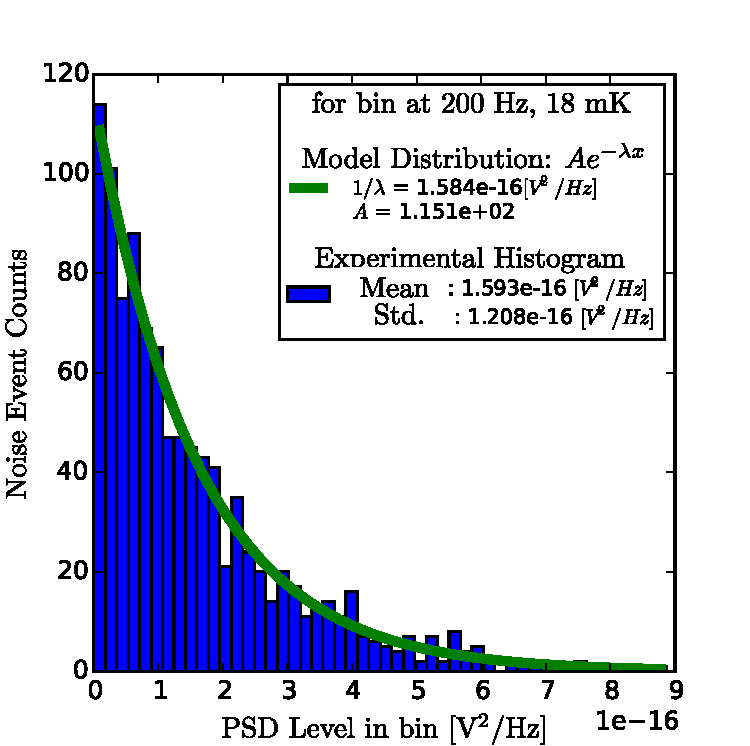
\includegraphics[width=0.6\textwidth]{Figures/Ethem/fit_exp_fin.pdf}
\end{center}
\caption{Histogram of the noise PSD level in the frequency bin at \SI{200}{\Hz} adjusted by an exponential model.}
\label{fig:noise-form}
\end{figure}

In a first step, the histogram of the measured PSD value for different frequencies is plotted. Such a histogram is presented as an illustration for a bin in frequency at \SI{200}{\Hz} on the figure \ref{fig:noise-form}. Regardless of the frequency probed, the temperature of the cryostat, or the electronics used, a similar distribution pattern is observed. An exponential distribution is successfully fitted to these histograms. A property of the exponential distribution can be applied to the noise: the mean PSD level $\mathcal{D}_i$ in the $i$-th frequency bin is equal to its standard deviation $\sigma_{\mathcal{D}_i}$. Indeed, the experimental values of the mean and the standard deviation are close to the term $1/\lambda$.
Thus, on a measure averaged over $N=120$ windows of $1$ second, the Central Limit Theorem expresses the standard deviation on the averaged measure $\sigma_{\bar{\mathcal{D}}_i}$ such that:
\begin{equation}
\label{eq:sigma-psd}
\sigma_{\bar{\mathcal{D}_i}} = \frac{\sigma_{\mathcal{D}_i}}{\sqrt{N}} = \frac{\bar{\mathcal{D}_i}}{\sqrt{120}}
\end{equation}

This information on the noise PSD   allows to rigorously construct a likelihood function based on the $\chi^2$ function related to the noise model with the set of parameters $\Theta$ and the experimental data $\mathcal{D}$.The expression of the $\chi^2$ function is:
\begin{equation}
\label{chi2}
\chi ^2 (\Theta|\mathcal{D}) = \sum^{N_{Temp}}_{j} \sum^{N_{bin}}_{i} \left[ \frac{\bar{\mathcal{D}_{ij}} - \mathcal{M}(f_{ij}; \Theta)}{\sigma_{\bar{\mathcal{D}_{ij}}}} \right]^2
\end{equation}
where we sum over all the frequency bins $N_{bin}$ and over the set of measurement temperatures $N_{Temp}$. Indeed, the model is simultaneously adjusted on several PSD measurements carried out for temperatures ranging from \SI{18}{\milli\kelvin} to \SI{40}{\milli\kelvin}. We thus hope to obtain better constraints on the parameters, firstly because more points are analyzed, but above all because the change in temperature modifies the system parameters (in particular the resistance of the NTD $R(T_e)$) and removes the problems of degeneration between the different free parameters.

Motivated by a Bayesian approach \cite{Billard:2012}, the likelihood function to be maximized with the model adjustment to the experimental data is expressed as,
\begin{equation}
\label{likelihood}
\mathcal{L}(\Theta | \mathcal{D}) = \exp{\left(\frac{-\chi ^2 (\Theta|\mathcal{D})}{2}\right)}
\end{equation}

\subsection{Monte Carlo Markov Chain Analysis }
\label{par:mcmc}
\label{sec:ethem-noise}
\label{par:ethem-noise}

We look for the set of parameters $\Theta$ that maximizes the likelihood function $\mathcal{L}(\Theta | \mathcal{D})$. To do this, we apply a Markov Chain Monte Carlo (MCMC) analysis with the use of the Python module "emcee" \cite{2013PASP}.
It is a method based on a random walk of one (or more) Markov chain, a set containing the free parameters, in the dimensional space $N=7$ corresponding to the number of free parameters.
It has been shown that with a correct likelihood function, the Markov chain allows to sample this function in a neighborhood of the optimal solution. The advantages of the MCMC method are that it can probe a large part of the free parameter space and converges quickly to the neighborhood of the optimal solution which can then be explored and analyzed with histograms of Markov chain positions. Figure \ref{fig:triangle-mcmc} displays such histograms in the case of the adjustment to the noise PSD of the \Edelweiss{} electronics.
\begin{figure}
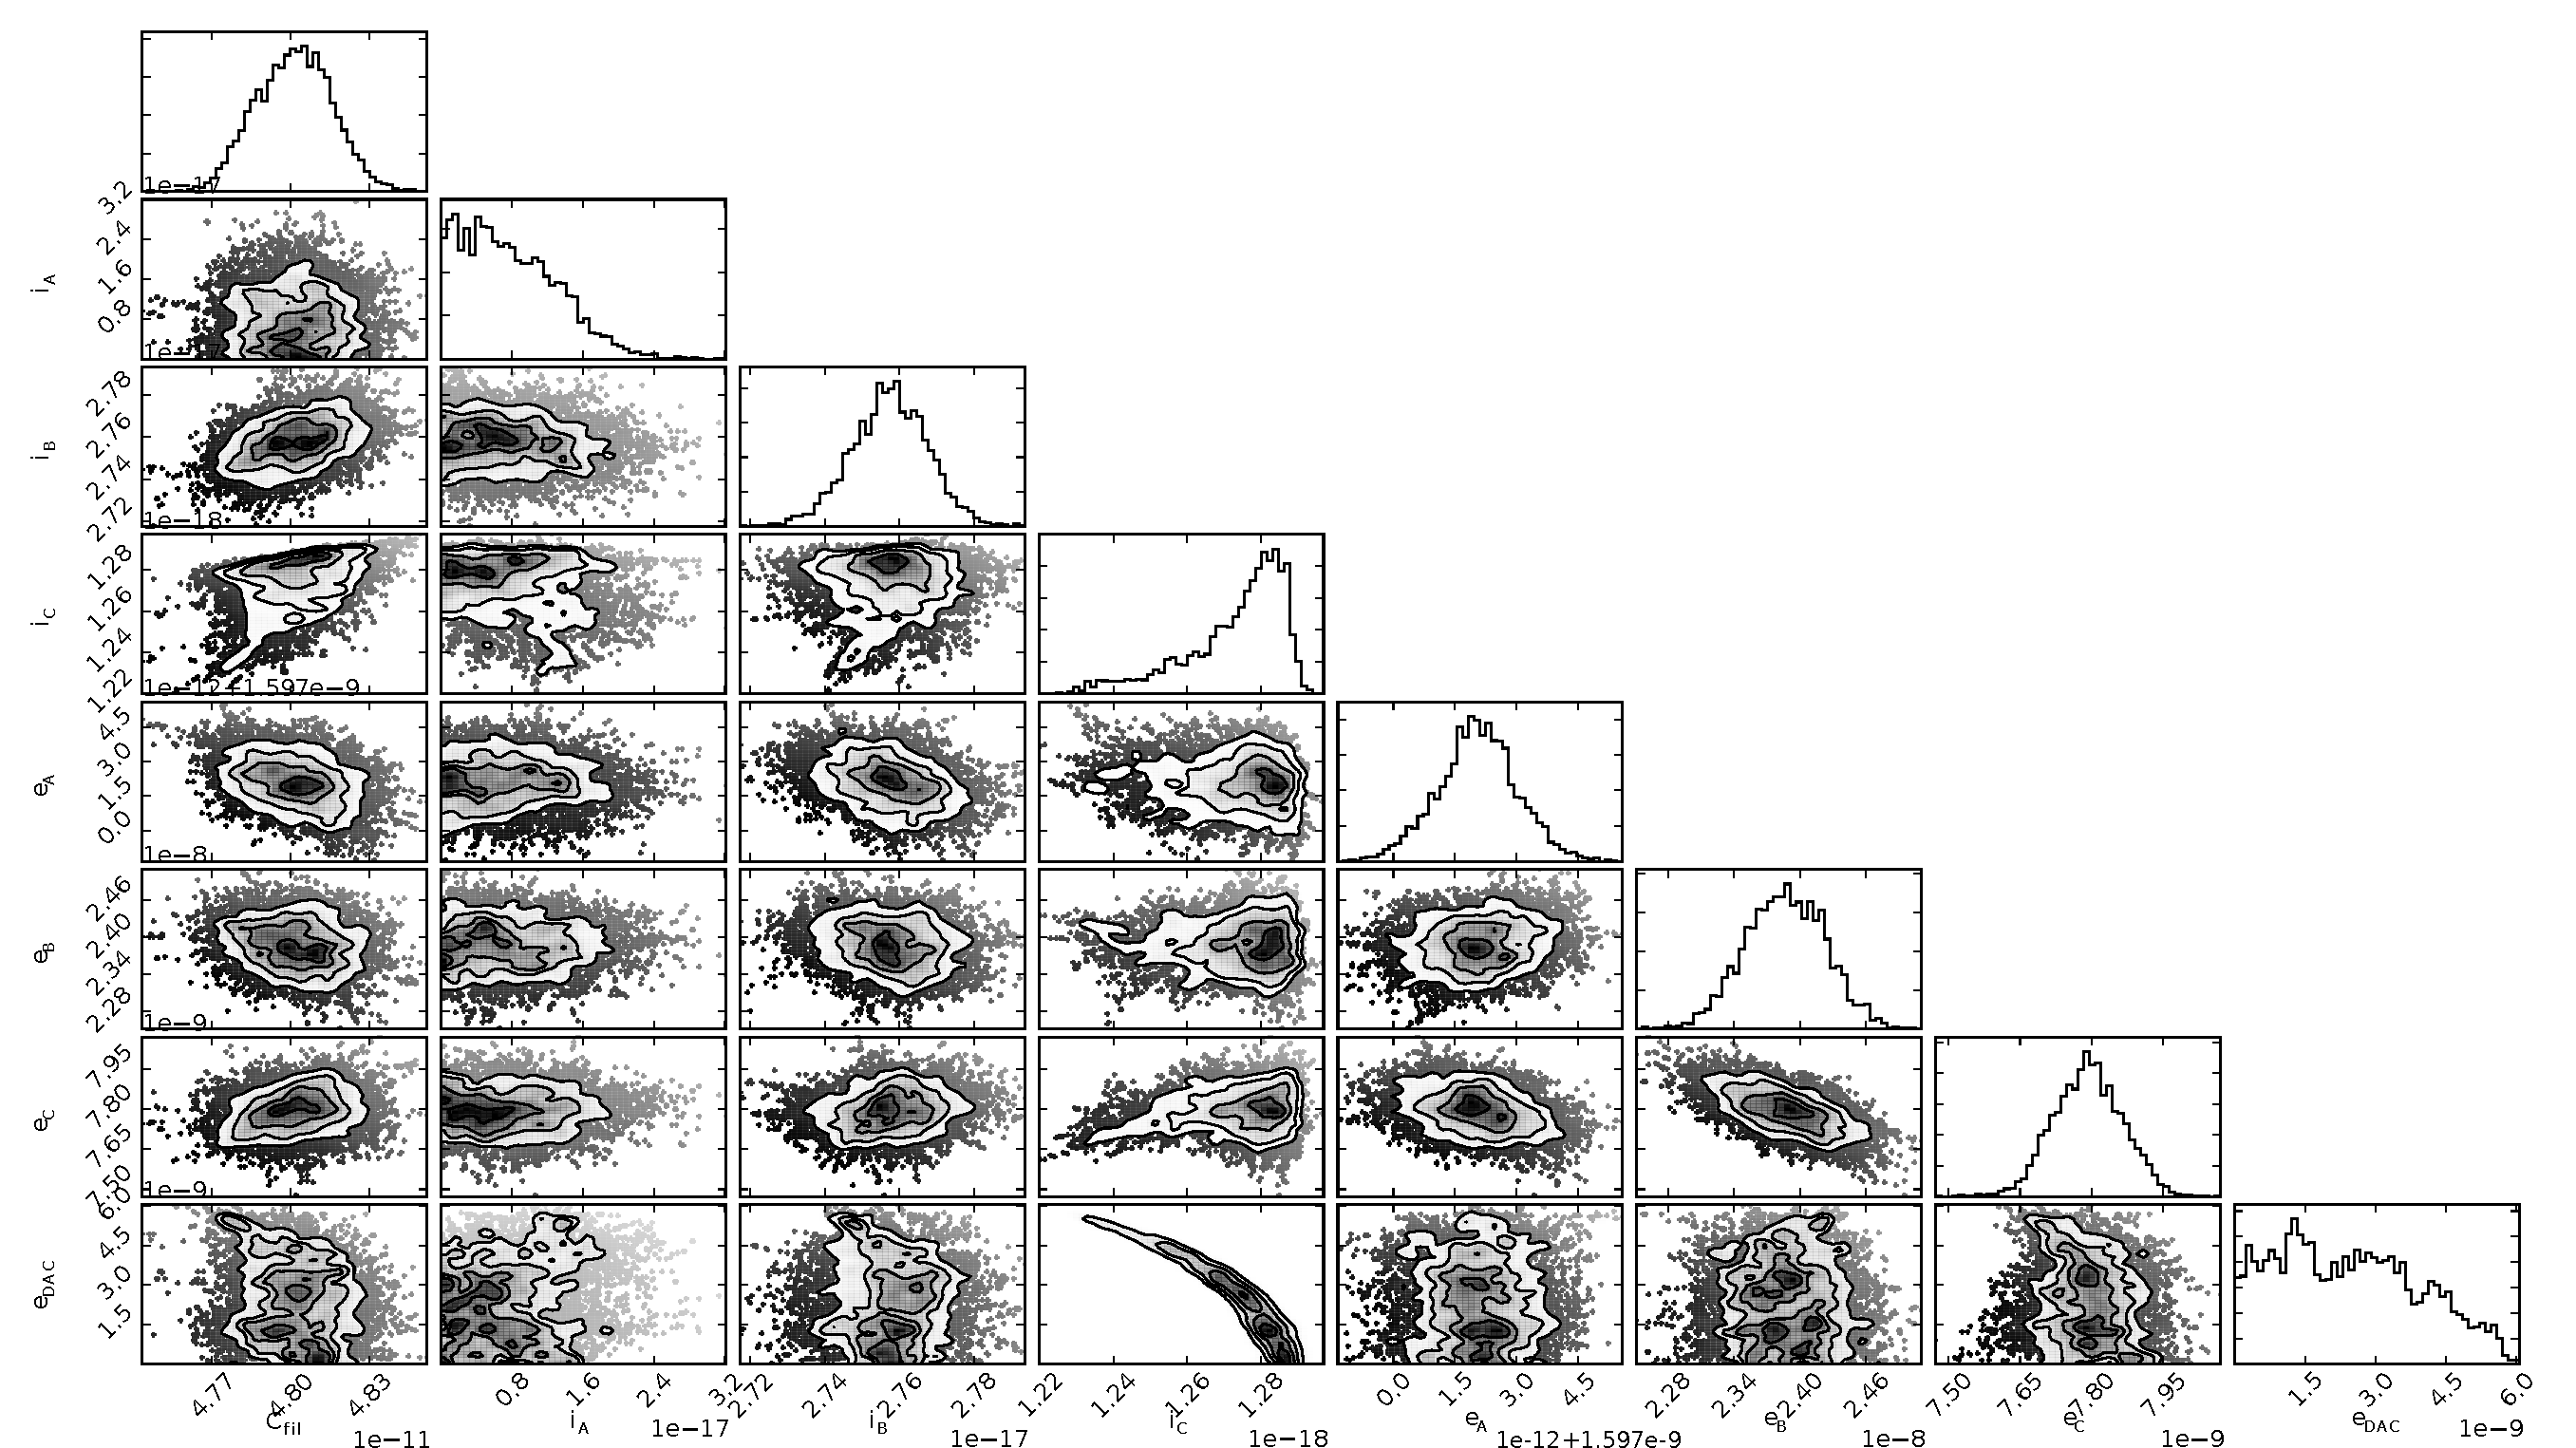
\includegraphics [width=\textwidth]{Figures/Ethem/triangle_fin.pdf}
\caption{Histogram of Markov chain positions with 2-dimensional projections, during MCMC analysis for \Edelweiss{} electronics. The free parameters presented are from top to bottom, and from left to right: $C_{cabling}, i_A, i_B, i_C, e_A, e_B, e_C, e_{DAC}$.}.
\label{fig:triangle-mcmc}
\end{figure}
From the position histogram, the mean position is extracted as an estimate of the set of optimal free parameters as well as the $1\sigma$ error bars on this estimate from the 0.16 and 0.84 quantiles of the distributions. The shape of the distributions also informs us about the quality of the constraint imposed on the considered parameter. Indeed, a narrow distribution indicates a well constrained parameter (like parameter $i_B$) with small error bars contrary to a distribution with wide spread which induces large error bars (like parameter $i_A$). Two parameters whose projection in 2 dimensions is elongated indicates their correlation (parameter $i_C$ and $e_{DAC}$).

\begin{figure}
\begin{center}
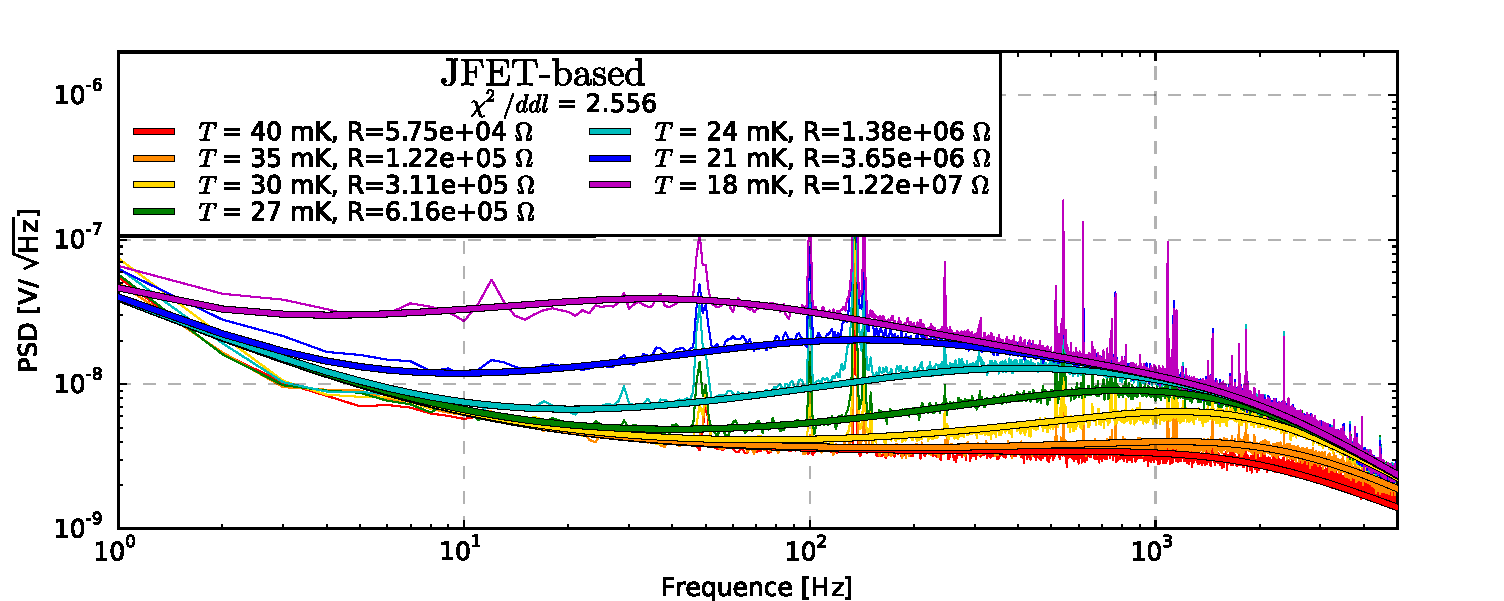
\includegraphics[width=\textwidth]{Figures/Ethem/cuore_fit_fin.pdf}
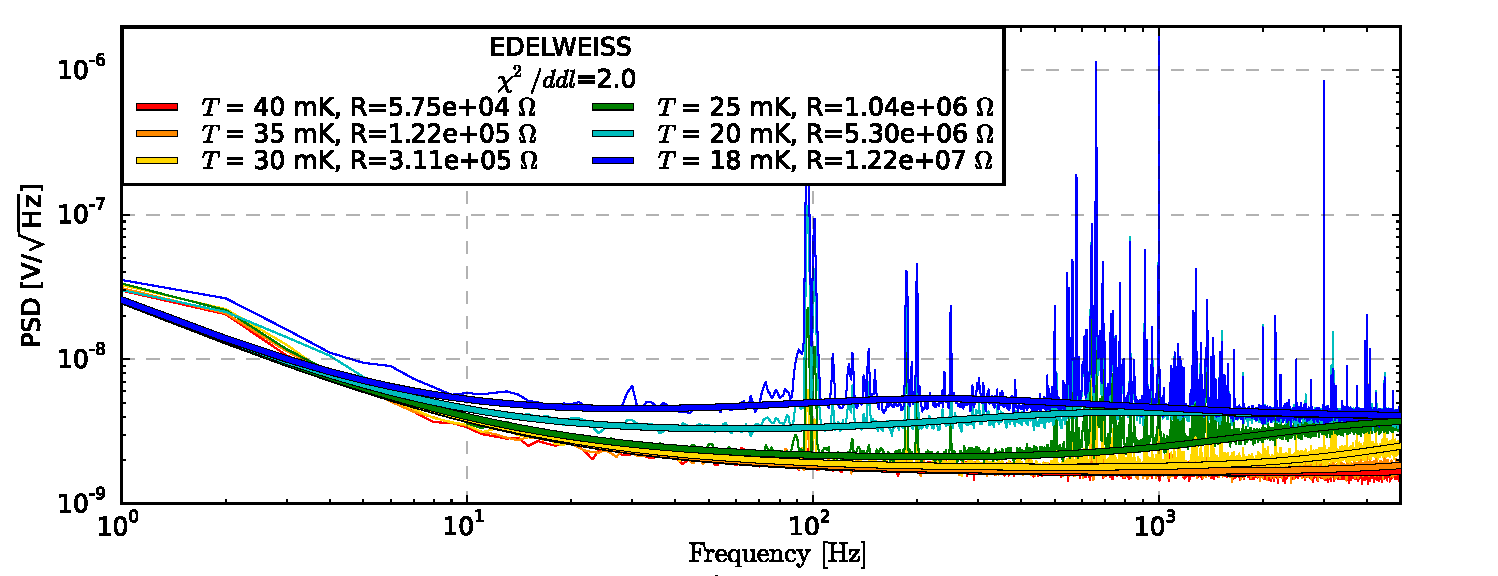
\includegraphics[width=\textwidth]{Figures/Ethem/edel_fit_fin.pdf}
\end{center}
\caption{Averaged measurements (thin lines) and adjustment by MCMC analysis (thick lines) of noise linear PSD for different temperatures on both electronics: JFET-based and \Edelweiss{}. It is important to note that these are noise measurements performed without polarization current. For each cryostat temperature $T$ is specified the value of the thermistor $R$. The term $\chi^2/ddl$ indicates the value of the function $\chi^2$ divided by the number of points (degrees of freedom) of the fit. For a perfect modeling of the experimental data: $\chi^2/ddl \rightarrow 1$}
\label{fig:rainbow-plot}
\end{figure}

After MCMC analysis, we obtain the fit of the experimental data related to JFET-based and \Edelweiss{} electronics presented in the figure \ref{fig:rainbow-plot}. The adjustment was performed on the PSD envelope, the parasitic peaks were ignored for the analysis. For the JFET-based electronics, a cut-off above \SI{2}{\kilo\Hz} is observed: this comes from a low-pass filter integrated in the electronics. It has been taken into account and therefore does not affect the convergence of the MCMC for this electronics. We also note the appearance of two additional free parameters. The $f_B$ parameter corresponds to the order of the low-pass filter for JFET-based measurements. The parameter $e_{DAC}$ corresponds to the noise of a power supply connected in series with the capacitance of the \Edelweiss{} electronics. 
%These additional parameters give more flexibility to the model so that it better adapts to the experimental data, and thus does not distort the optimal solution.

We check that the fit is excellent over all frequencies, with some slight difference in behavior for the low frequencies of the JFET-based electronics. Indeed, the function of $\chi^2$ weighted by the number of degrees of freedom $ddl$ is equal to $2.556$ for JFET-based and $2.0$ for \Edelweiss{}, which is close to the value $1$ corresponding to a perfect modeling. The optimal solutions, indicated in the table \ref{tab:result}, for the electronics allow to simulate the noise of the electronics from the proposed model of electronics noise (eq. \ref{eq:i-amplifier} and \ref{eq:e-amplifier}). Different behaviors are observed depending on the temperature of the cryostat: the PSD levels are globally larger at low temperatures. This can be explained by the contribution of the current noise $i_{noise}$ increasing with the norm of the complex impedance $Z_{eq}$. Indeed, the NTD resistance $R(T_e)$ increases very strongly when the temperature of the cryostat decreases, so the complex impedance $Z_{eq}$ also increases.

\begin{align}
\label{tab:result}
\begin{aligned}[c]
& \textrm{\textbf{JFET-based}} \\
C_{fil} &= (2.94 \pm 0.01)\times 10^{-10}&[F] \\
i_A &= (1.9 \pm 0.03) \times 10^{-15}&[A/\sqrt{Hz}] \\
i_B &= (6.11 \pm 0.01) \times 10^{-16}&[A/Hz] \\
i_C &= (1.16 \pm 0.01) \times 10^{-17}&[A/Hz^{3/2}] \\
e_A &= (3.28 \pm 0.01) \times 10^{-9} &[V/\sqrt{Hz}] \\
e_B &= (3.03 \pm 0.04) \times 10^{-8}&[V] \\
e_C &= (1.08 \pm 0.02) \times 10^{-8} &[V \cdot \sqrt{Hz}] \\
f_B &= (2.70 \pm 0.01) & [u.a.]
\end{aligned}
\quad \vrule{} \quad
\begin{aligned}[c]
& \textrm{\textbf{EDELWEISS}} \\
C_{fil} &= (4.80 \pm 0.02)\times 10^{-11}&[F] \\
i_A &= (6.17 \pm 4.8) \times 10^{-18}&[A/\sqrt{Hz}] \\
i_B &= (2.76 \pm 0.01) \times 10^{-19}&[A/Hz] \\
i_C &= (1.28 \pm 0.02) \times 10^{-18}&[A/Hz^{3/2}] \\
e_A &= (1.60 \pm 0.00) \times 10^{-9} &[V/\sqrt{Hz}] \\
e_B &= (2.39 \pm 0.04) \times 10^{-8}&[V] \\
e_C &= (7.81 \pm 0.07) \times 10^{-9} &[V \cdot \sqrt{Hz}] \\
e_{DAC} &= (2.02 \pm 1.9) \times 10^{-9}&[V/\sqrt{Hz}] 
\end{aligned}
\end{align}

The low-frequency behavior of the two electronics is very similar: one observes a strong rise at low frequencies associated with the parameters $e_{B,C}$. At higher frequencies, we note that the JFET-based electronics noise PSDs are much more sensitive to temperature than for the \Edelweiss{} electronics. For all temperatures, the noise level of the JFET-based electronics is higher than that of \Edelweiss{}. We simply have a factor of 2 at \SI{40}{\milli\kelvin} while we have almost an order of magnitude difference at \SI{18}{\milli\kelvin}. The fitting parameters listed in table \ref{tab:result} show a difference of two orders of magnitude between the current noise $i_A$ of the two electronics. For the \Edelweiss{}, the current noise is coupled to the complex impedance $Z_{eq}$ which explains the measured noise level.

\begin{figure}
\begin{minipage}{0.49\textwidth}
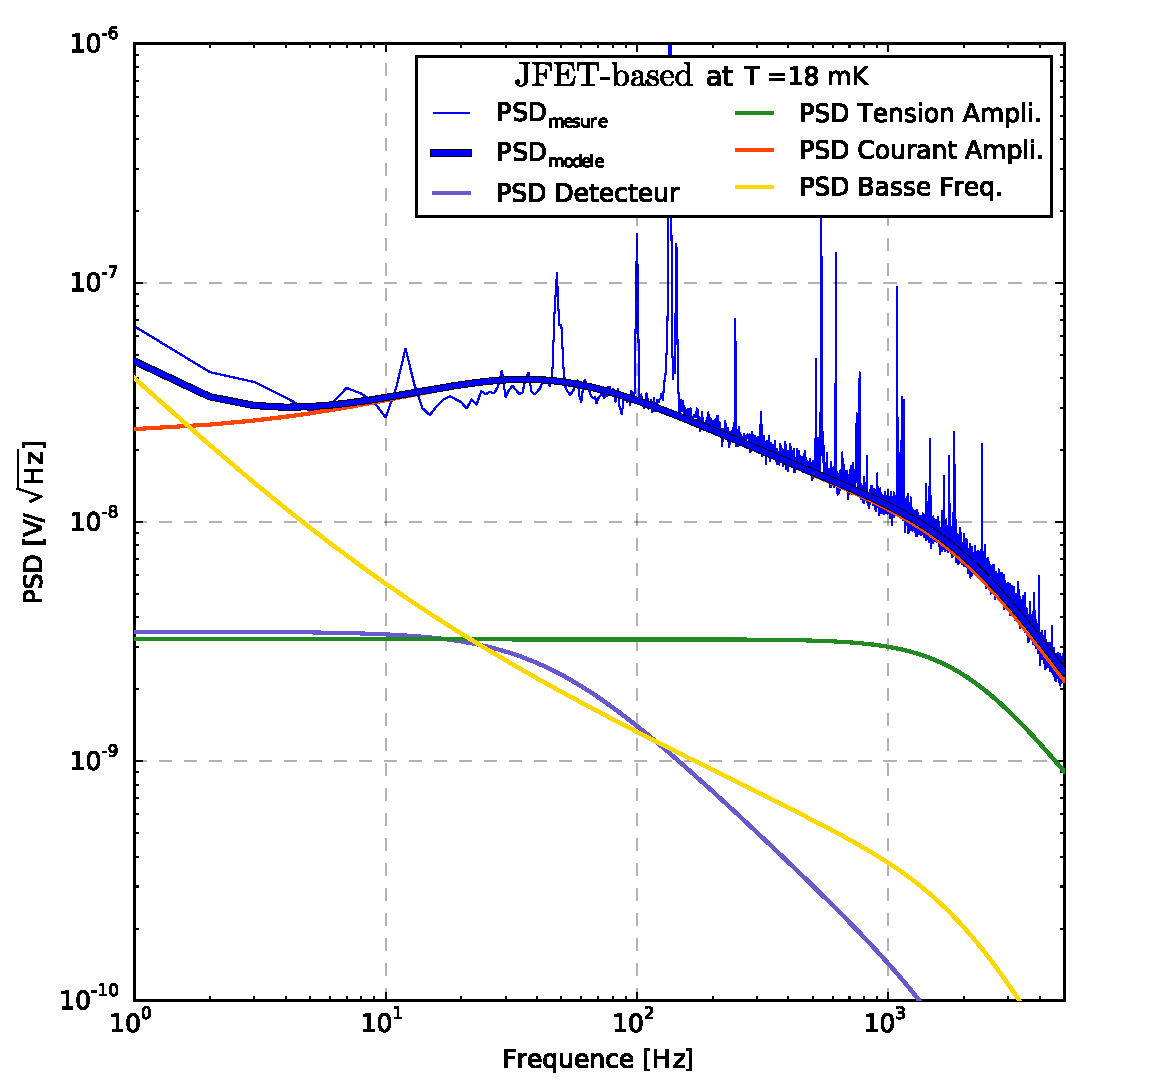
\includegraphics[width=\textwidth]{Figures/Ethem/cuore_18.pdf}
\end{minipage}
\hfill
\begin{minipage}{0.49\textwidth}
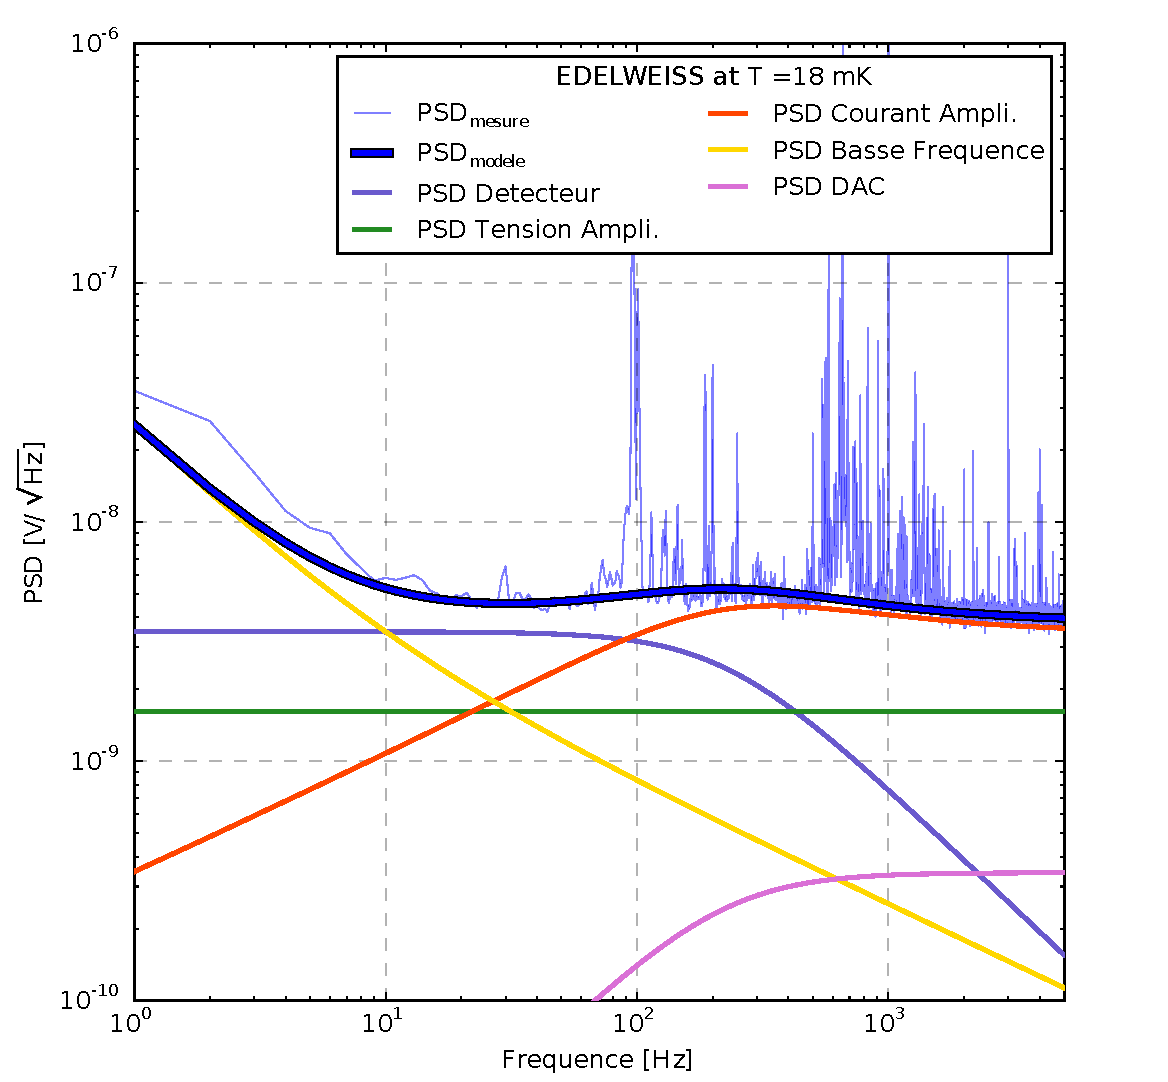
\includegraphics[width=\textwidth]{Figures/Ethem/edel_18.pdf}
\end{minipage}
\caption{Experimental measurement and model of a noise spectral density at $18$ mK for JFET-based (left) and \Edelweiss{} (right) electronics with visualization of the contributions of the different noise sources.}
\label{fig:noise-sources}
\end{figure}

It therefore appears that the least noisy is the \Edelweiss{} electronics. It is thus with this electronics that it is agreed to optimize the resolution of the detectors. 
%Nevertheless, at the time of this study, the \Edelweiss{} electronics was not ready to readout the heat channel in in the same time polarizing the NTD thermal sensor. Only the JFET-based electronics was available for heat measurements with polarization to characterize the RED10 detector. As it has also been characterized, this does not generate any particular issue.

Using the optimal solution found with the MCMC analysis, it is possible to visualize the contributions of the different noise sources to the total noise PSD, an example at \SI{18}{\milli\kelvin} is shown in figure \ref{fig:noise-sources} for the two electronics. It can be seen that the current noise of JFET-based is very high and dominates almost the whole frequency range. The Johnson noise cut-off frequency, which is different for the two electronics, illustrates the influence of the cabling capacitance $C_{cabling}$. Indeed, we have $f_{cut} = 2\pi/(R_{NTD} C_{cabling})$ considering $R_L\gg R_{NTD}$. A higher cut-off frequency is found in the case of \Edelweiss{} which has a lower cabling capacitance according to the fitting parameters (eq. \ref{tab:result}). It is also possible to study the predominance of noise sources as a function of frequency. For the electronics of \Edelweiss{}:
\begin{itemize}
\item below \SI{10}{\Hz}, the noise is dominated by the low-frequency contributions of noise in voltage $e_{B,C}$.
From \SI{10}{\Hz} to \SI{100}{\Hz}, the total noise is based on the intrinsic noise of the detector (TFN noise and Johnson noise of the NTD). This is exactly what is sought: one seeks to be limited by these detector thermal noises which sets the ultimate attainable limit.
\item above \SI{100}{\Hz}, the current noise of the amplification electronics characterized by the coefficients $i_{A,B,C}$ becomes predominant.
\end{itemize} 


\subsection{Calculation of the NEP and Resolution}
\label{par:nep-res}

Now that we have constrained all the parameters of the noise model, it is possible to finalize the computation of the resolution (eq. \ref{eq:resolution}) with the computation of the NEP (eq. \ref{eq:nep}). Figure \ref{fig:nep-fig} shows the simulated sensitivity and NEP graphs of the detector for the \Edelweiss{} electronics at \SI{18}{\milli\kelvin} for a bias current $I_P = \SI{1}{\nano\ampere}$. The sensitivity is consistent with the transfer function of a thermal system: it is indeed a low-pass. The simulation of the NEP is obtained from the sensitivity and the total noise PSD according to the formula \ref{eq:nep}. It presents its lowest values between \SI{1}{\Hz} and \SI{100}{\Hz}. 

\begin{figure}[!ht]
\begin{minipage}{0.49\textwidth}
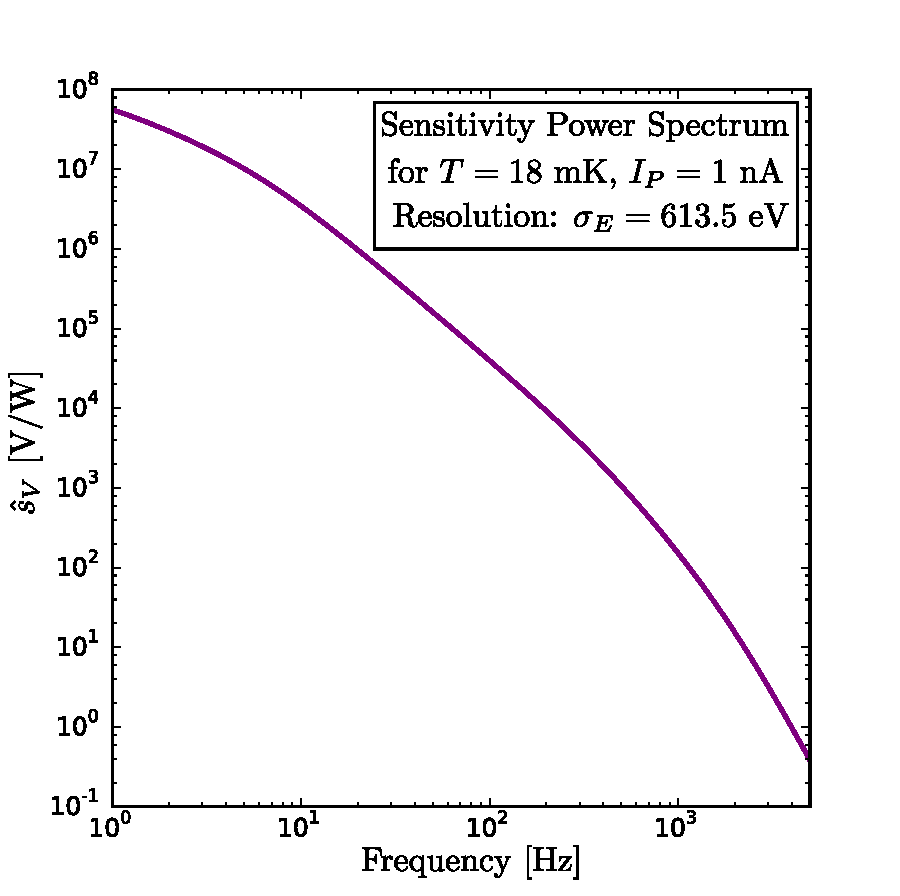
\includegraphics[width=\textwidth]{Figures/Ethem/sv_fin.pdf}
\end{minipage}
\hfill
\begin{minipage}{0.49\textwidth}
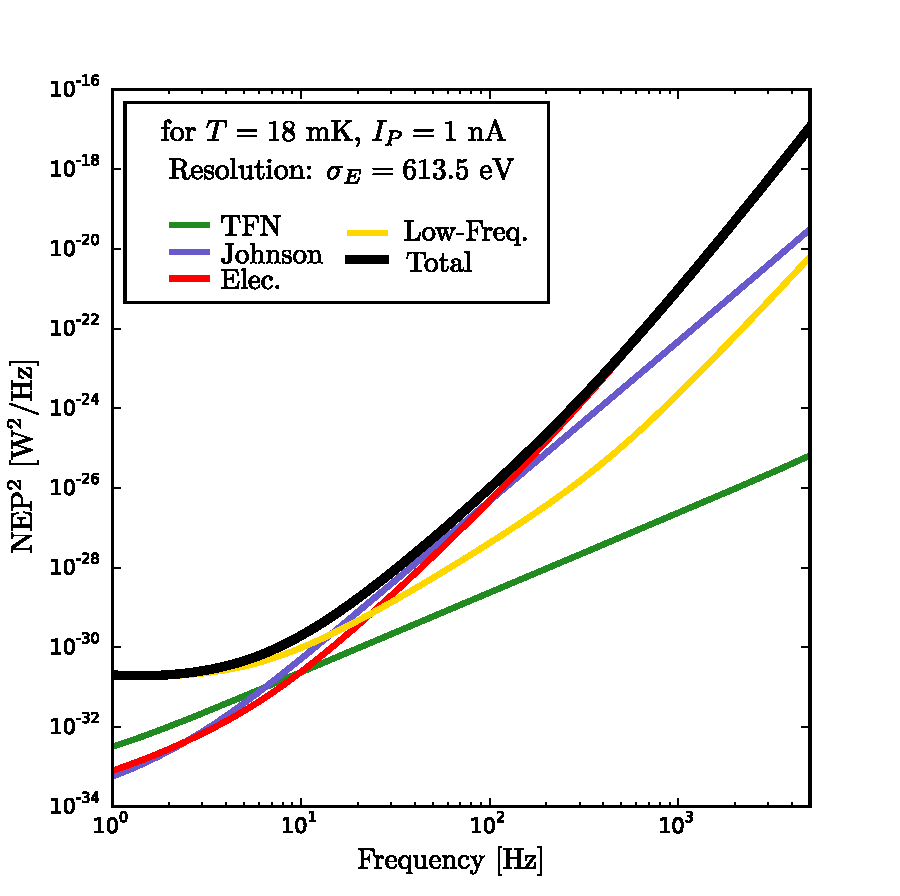
\includegraphics[width=\textwidth]{Figures/Ethem/nep_fin.pdf}
\end{minipage}
\caption{Simulation of sensitivity (left) and NEP (right) with contributions of different noise sources for \Edelweiss{} electronics at a cryostat temperature of $T=18$mK and a bias current of $1$nA.}
\label{fig:nep-fig}
\end{figure}


It is now possible to access the resolution of this experimental configuration with the associated formula \ref{eq:resolution}. We calculate here a heat energy resolution of $\sigma_E = \SI{613.5}{\eV}$ for \Edelweiss{}, and a resolution of \SI{1061}{\eV} with the JFET-based electronics, with a temperature of \SI{18}{\milli\kelvin} and a bias current of \SI{1}{\nano\ampere}. A lower value is obtained with the \Edelweiss{} electronics, which further confirms the choice of this electronics for the optimization of the resolution.

The formula \ref{eq:resolution} used for calculating the resolution indicates that the lowest NEP values contribute the most to the resolution. Although integrating over a wider frequency range results in lower resolution, the gain becomes negligible as the NEP value increases.
Note that the NEP takes its minimum values around \SI{10}{\Hz}: most of the heat measurement information is contained in a frequency range from \SI{0}{\Hz} to about \SI{50}{Hz}. The gain in resolution by integrating beyond \SI{50}{\Hz} is marginal. The frequency range of interest for the study of the signal is then identified. By observing the contributions of the different noise sources to the NEP in figure \ref{fig:nep-fig}, we can see that it is the low frequency (LF) noise that dominates in this frequency range of interest, followed by the Johnson noise of the NTD resistor. We understand that to further decrease the resolution of these detectors, we should increase the sensitivity of the system to an event or reduce this low-frequency noise. %Part of the MANOIR team is already working to understand this low-frequency noise.



% HERE
\subsection{Thermal Characterization of the RED10 Detector}

At the time of this study of the heat channel, the RED10 detector had only recently come into the possession of the MANOIR group. It shares its design with the prototype RED1. The difference with the latter lies in the glue composition used and the dimensions of the NTD used. Some thermal parameters are therefore modified compared to RED1. It is thus necessary to characterize these thermal parameters for this new detector. One will be able to study its response to an event as it was done with RED1 in the previous section.

\subsection{Current-Voltage Characteristic and Signal Shape}

The characterization of the thermal parameters uses the electro-thermal model that was built in the section \ref{sec:electro-thermal-model}. We want to adjust the unconstrained parameters to the experimental data with an MCMC analysis similarly to the characterization of the electronics in the subsection \ref{par:mcmc}. This time, the set of free parameters is:
\begin{equation}
\Theta = (R_0, T_0, g_{ep}, g_k, g_{glue}, \epsilon, \tau_P)
\label{theta-red10}
\end{equation}
Indeed, the new glue has a different conductivity $g_{glue}$. The new geometry of the NTD (and also its uncertainty of neutron doping) will lead to a modification of the resistance $R_0$ and characteristic temperature $T_0$ present in the equation \ref{eq:ntd-resistivity}. The change in dimension also impacts the electron-phonon coupling $g_{ep}$ and the Kapitza conduction coefficient $g_k$. In principle, the volumetric thermal capacities of the absorber and the NTD remain unchanged, which makes it possible to recalculate the new thermal capacities from the known dimensions of the NTD. It would have been possible to include these in the free parameters, but the choice to fix them was favored in order to avoid degeneration problems and thus better constrain the set of parameters $\Theta$.

A preliminary study of the signal shape (shown on the right of figure \ref{fig:v2i-red10}) of RED10 reveals that the pulse decay has two characteristic time constants. This type of signal has never been observed on signal measurements performed with RED1: there is only one characteristic decay time explained by the thermal leakage to the cryostat from the electron bath with a recoil energy deposit in the absorber. The presence of a second characteristic time for RED10 can only be explained by the presence of athermal phonons as introduced in section \ref{par:ethem-frequency-domain}. These are phonons that do not immediately relax in the absorber, pass into the NTD sensor before relaxing. They thus create a temperature rise directly within the NTD. The source term $\bm{F}$ in the equation \ref{eq:ethem-coupling-mat} is then rewritten:
\begin{equation}
\label{eq:source-athermal}
\bm{F}(t-t_0) = 
\left( \begin{array}{c}
(1-\epsilon)E/C_a \\
0 \\
\epsilon E/C_e \\\
0
\end{array} \right) \delta (t-t0)
\end{equation}
with $\epsilon$ the fraction of recoil energy converted into athermal phonons, and $C_a$ and $C_e$ the thermal capacity of the absorber and the electron bath respectively.

The normalization constants of the general time solution (eq. \ref{eq:eigein-solution-expr}) depend on the source term $\bm{F}$ according to formula \ref{eq:ethem-initial-value} and therefore differ from the case of RED1, devoid of athermal phonons. This has the effect of better expressing a new exponential, and thus a new characteristic time, contained in the general solution. This observation of two characteristic times for the signal motivates the addition of the fraction of athermal phonons $\epsilon$ and their characteristic relaxation time $\tau_P$ to the free parameters of the model.

The electro-thermal model is adjusted to the experimental data collected with RED10. The detector RED10 is polarized with a fixed bias current $I_P = \SI{4}{\nano\ampere}$ for different temperatures ranging from \SI{18}{\milli\kelvin} to \SI{30}{\milli\kelvin}. We study the behavior of RED10 in the steady state (see section \ref{par:steady-state}), with its experimental current-voltage characteristic, and its temporal response (section \ref{par:time-domain}) with experimental heat signals generated by electronic recoils induced by the natural radioactivity. The likelihood function analysis is performed with the MCMC method as in section \ref{par:mcmc}. Experimental data with the adjusted models are presented in the figure \ref{fig:v2i-red10}.

\begin{figure}
\begin{minipage}{0.49\textwidth}
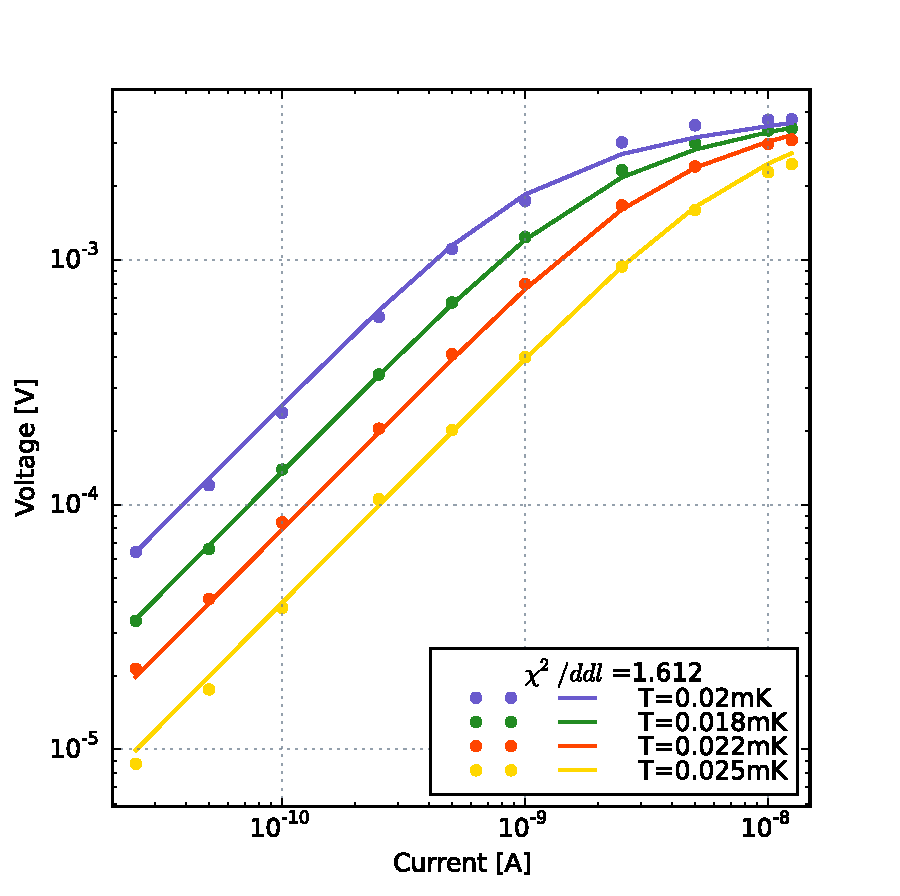
\includegraphics[width=\textwidth]{Figures/Ethem/v2i_red10.pdf}
\end{minipage}
\hfill
\begin{minipage}{0.49\textwidth}
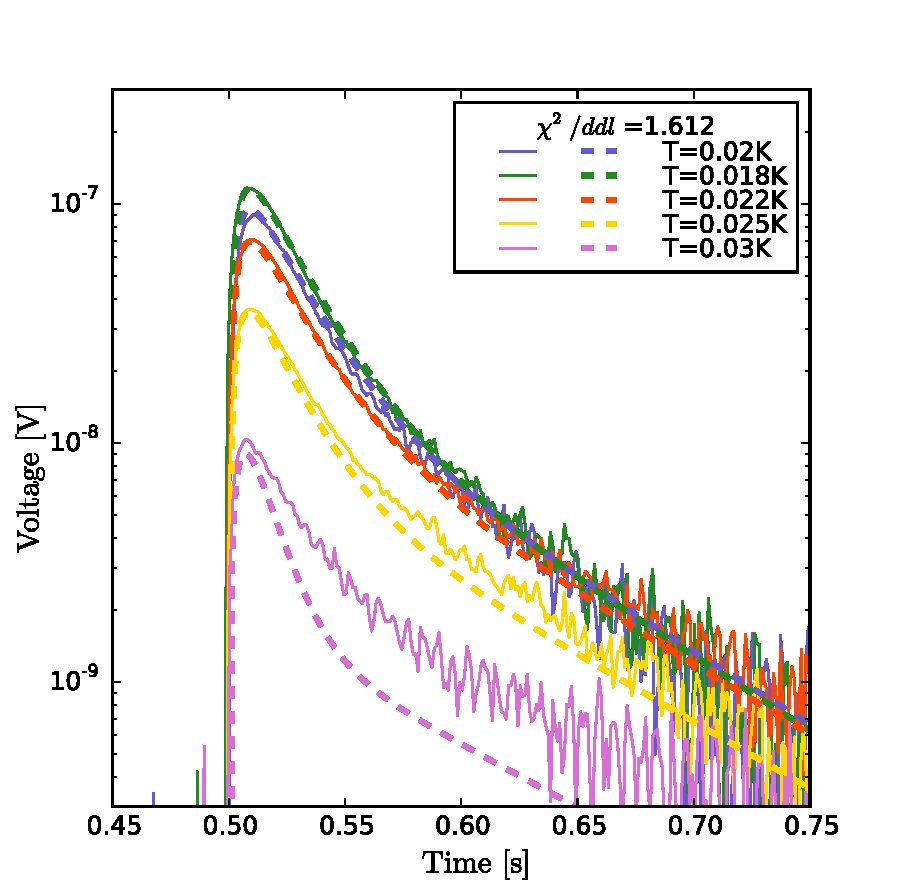
\includegraphics[width=\textwidth]{Figures/Ethem/pulse_red10.pdf}
\end{minipage}
\caption{Experimental measurements and model fittings of the current-voltage characteristic (left) and normalized heat signals (right) for the RED10 detector.}
\label{fig:v2i-red10}
\end{figure}

The fit seems good for both types of measurement with a $\chi^2/ddl=1.612$. However, the model has some difficulty in adjusting the pulse at a temperature of \SI{30}{\milli\kelvin}. The current-voltage characteristic, also called V(I) curve, makes it possible to constrain the free parameters involved in the steady state equations \ref{eq:ethem-system-stationnary}: $R_0, T_0, g_{ep}, g_k$. The experimental points in the linear part of the V(I) curves below \SI{1}{\nano\ampere} mainly constrains the resistance value of the NTD, and thus $R_0, T_0$. The voltage plateau at higher bias current above \SI{1}{\nano\ampere} comes from an excessive Joule effect in the NTD which is then no longer compensated by the thermal leakage to the cryostat. The temperature of the NTD increases and its resistivity decreases with constant bias current $I_P$, which causes the voltage plateau to appear. Its adjustment thus constrains the values of conductivity $g_k$ and electron-phonon coupling $g_{ep}$.

As for the shape of the signal, the model shows two slopes and thus two characteristic times. The adjustment of these two decay slopes constrains the athermal phonon fraction $\epsilon$, and more generally, all the parameters involved in the calculation of the normalization constants of the time dependent solutions \ref{eq:eigen-solution}.
The rise in tension allows to constrain the relaxation time of the phonons $\tau_P$. Indeed, for an immediate relaxation of the phonons, the rise time would be infinitely large (modulo the cutoff frequency $(RC_{cabling})^{-1]}$).

The MCMC method then gives the fitting parameters for RED10:

\begin{align}
R_0 &= (11.6 \pm 0.4)&[\Omega] \\
T_0 &= (2.72 \pm 0.01) &[K] \\
g_{ep} &= (21.1 \pm 4.4) &[W/K^6/cm^3] \\
g_k &= (2.77 \pm 0.1) \times 10^{-4}&[W/K^4/mm^2] \\
g_{glue} &= (7.46 \pm 1.67) \times 10^{-4} &[W/K^{n_g}/mm^2] \\
\epsilon &= (0.202 \pm 0.001)  & [fraction]\\
\tau_P &= (4.03 \pm 0.03) \times 10^{-3} &[s]
\end{align}

These values are of the same order of magnitude as those corresponding to RED1. It is important to highlight the high portion heat energy expressed as athermal phonons of about \SI{20}{\percent} which is to be compared to their complete absence within the RED1 detector. This is a new observation for this type of detector. Their high proportion results in an acceleration of the voltage signal and thus an increase of the frequency range of interest of the signal introduced in section \ref{par:nep-res}. In addition, athermal phonons are not affected by the capacity of the absorber, and transmit all their energy directly to the NTD. Understanding and increasing the rate of athermal phonons will thus allow to increase the sensitivity leading to lowered energy resolution of the detector. A new way of optimizing the detectors has been discovered, which has not yet been considered within the R\&D program.


\subsection{Noise Levels and Energy Resolution of RED10}

Since RED10 is fully characterized from the thermal point of view, and the JFET-based electronics used for the measurements is also characterized, we are able to simulate the noise spectrum related to RED10 compared to the experimental measurement. Figure \ref{fig:noise-red10} shows the adjusted model and the experimental measurement of the noise PSD of RED10 for a bias current of \SI{4}{\nano\ampere} and an operating temperature of \SI{22}{\milli\kelvin}. Note that a Bessel filter is applied to the measurement, and to the model, which explains the cutoff appearing from \SI{2}{\kilo\Hz}.

\begin{figure}
\begin{center}
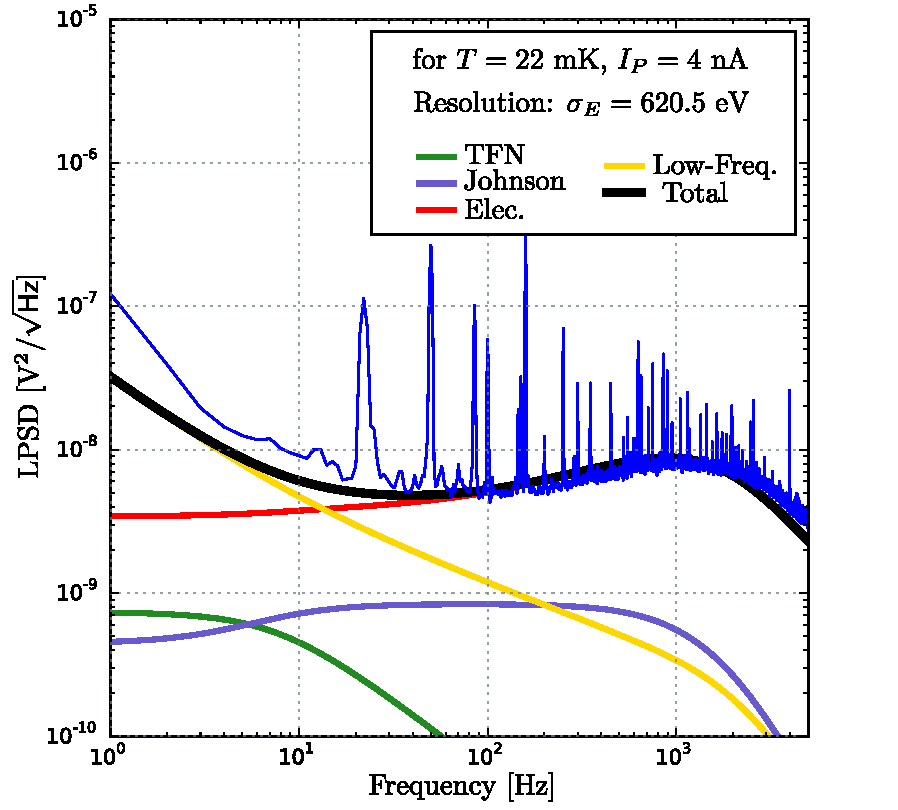
\includegraphics[width=0.55\textwidth]{Figures/Ethem/modexp.pdf}
\end{center}
\caption{Experimental measurement of the noise PSD at $22 mK$ with RED10 compared to its simulation with the electro-thermal model.}
\label{fig:noise-red10}
\end{figure}

The model and the measurement describe very similar developments. We do find the presence of a low frequency noise of high level dominating the total noise PSD up to \SI{15}{\Hz}. It is then the current noise that predominates over the rest of the frequency range.
It should be noted that this PSD measurement is performed with the polarization of the NTD as opposed to the characterization of the noise of the JFET-based and \Edelweiss{} electronics which was done with $I_P = \SI{0}{A}$. As such, it would be incorrect to compare the presented current noise of RED10 with the current noise of RED1 obtained without bias current.
There is a slight shift in the model from the experimental data to the low frequencies. This can be explained by the underestimation of the low-frequency noise already observed for the JFET-based electronics in the figure \ref{fig:rainbow-plot}. The excess of low-frequency noise also comes from the high rate of muon events during the measurements: despite the cuts made in the analysis, part of the signal decay is always recovered, which helps to amplify the low frequencies of the measured spectrum.

The experimental resolution measurement is carried out from the noise PSD and the measurement of a heat signal. Indeed, renormalizing the amplitude of the signal and applying a Welch method allows to estimate the signal power spectrum, equivalent to the sensitivity $s_V$ of the RED10 detector. The renormalization also requires to know the conversion between the energy deposited in the absorber by an event and the amplitude of the measured signal. This calibration is performed using the interaction of cosmic muons with the absorber. The energy they deposit in the absorber is equal to \SI{18}{\mega\eV}. Measuring the voltage amplitude of a muon signal therefore allows to deduce the conversion factor necessary for the renormalization of a signal. The experimental heat energy resolution $\sigma_E$ is calculated using the discrete analogue of the formula \ref{eq:resolution}.

\begin{figure}[!ht]
\begin{center}
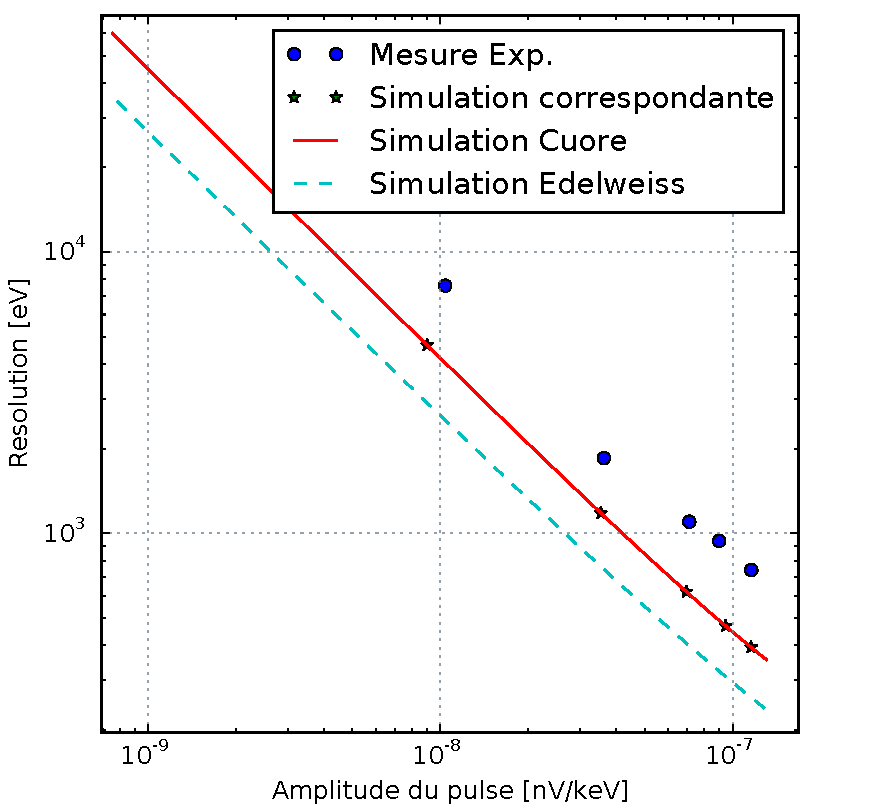
\includegraphics[width=0.55\textwidth]{Figures/Ethem/resamp_fin_fin.pdf}
\end{center}
\caption{Heat resolution $\sigma_E$ versus the normalized signal amplitude for the detector RED10 polarized with a bias current of \SI{4}{\nano\ampere}  with temperatures ranging from \SI{18}{\milli\kelvin} to \SI{30}{\milli\kelvin}.}
\label{fig:amp-res-red10}
\end{figure}

Figure \ref{fig:amp-res-red10} shows the energy resolutions $\sigma_E$ as a function of the normalized heat signal amplitudes in \si{\nano\volt\per\kilo\eV} for different temperatures at a fixed bias current. The experimental resolutions are higher than the simulated resolutions. This is explained by the deviation between model and noise measurement observed in figure \ref{fig:noise-red10}: the modeled low-frequency noise is lower than in reality, hence the simulation of lower resolutions. The pulse amplitude is used to estimate the sensitivity of RED10 to the signal. Except for the \SI{30}{\milli\kelvin} measurement where the signal was already poorly modeled, the simulated and real amplitude values are almost identical. Moreover, since the two sets of dots show a very similar evolution of the resolution as a function of amplitude, it is deduced that the model is in good adequacy with the experimental reality. A study of the noise difference is still necessary to obtain a complete adequacy of model and experiment.

It should be noted that the measurements were performed with the JFET-based electronics. The simulation of the resolution-amplitude characteristic is plotted for both the JFET-based and the \Edelweiss{} electronics. It should be noted that the latter makes it possible to gain almost a factor of 2 on the value of the resolution as the amplitude remains unchanged. This is consistent with the low noise level of \Edelweiss{} compared to the noise level of the common JFET-based electronics.


\subsection{Optimization of the RED10 Detector and Perspectives}

An electro-thermal model was built and tested with RED10. Even if some parameters need to be further refined to have a better fit, we can perform a preliminary optimization of the RED10 detector. A simulation of the resolution of RED10 as a function of the bias current $I_P$ in the NTD thermistance for different cryostat temperatures is presented in figure \ref{fig:optim}. The simulation is performed with the \Edelweiss{} electronics which has the lowest noise level, and the temperature of the load resistor is lowered to the temperature of the mixing chamber to reduce its Johnson noise.

\begin{figure}
\begin{minipage}{0.49\textwidth}
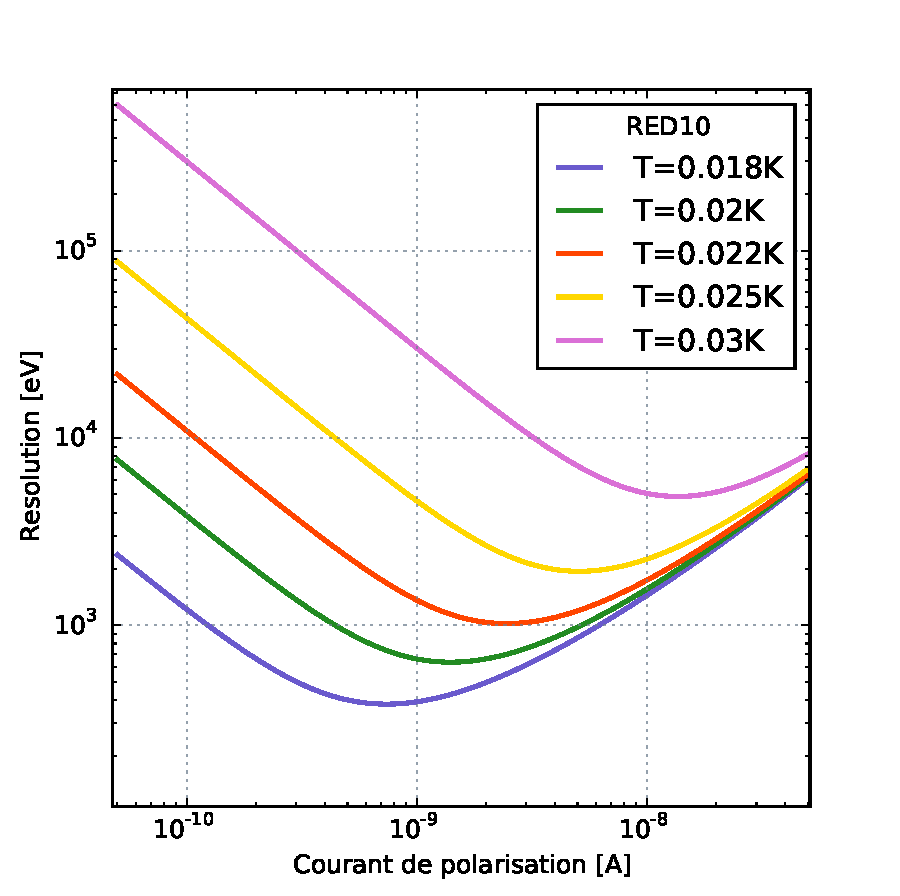
\includegraphics[width=\textwidth]{Figures/Ethem/red10_i.pdf}
\end{minipage}
\hfill
\begin{minipage}{0.49\textwidth}
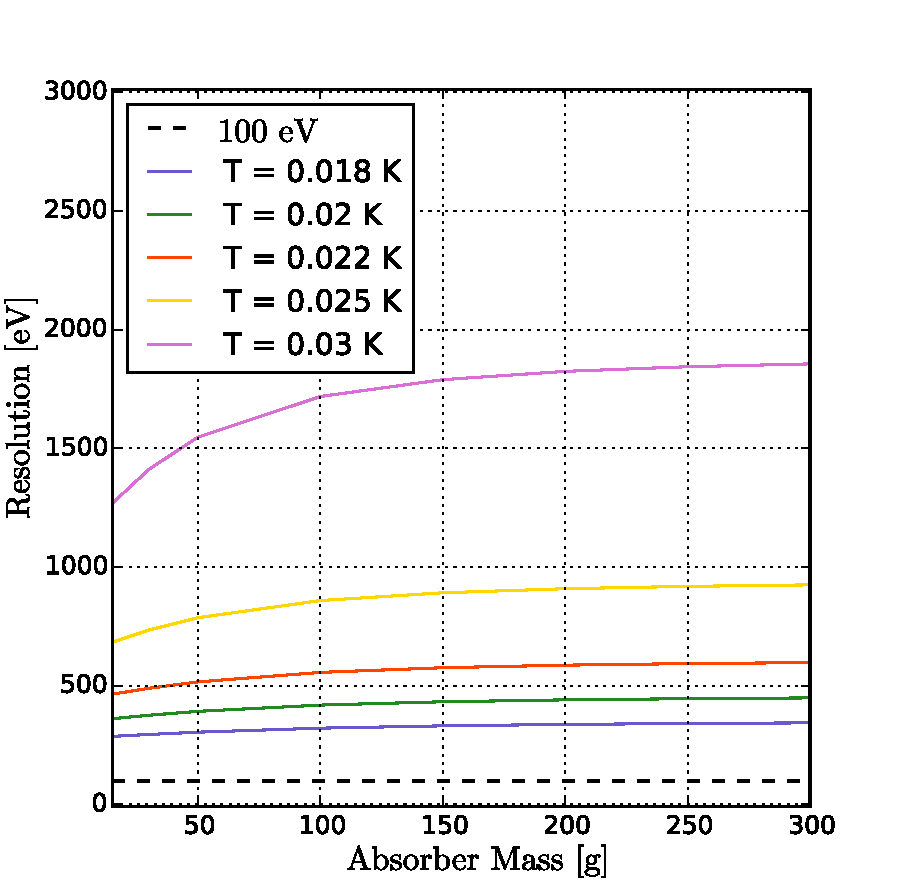
\includegraphics[width=\textwidth]{Figures/Ethem/red10_mass.pdf}
\end{minipage}
\caption{On the left, Simulation of the resolution of RED10 as a function of the bias current for different temperatures. On the right, Simulation of the resolution with optimized bias current as a function of the absorber mass for different temperatures. The design considered is the same as that of RED10, only the mass of the absorber is changed by adjusting the bias current to obtain the lowest resolution.}
\label{fig:optim}
\end{figure}

It is observed that there is an optimal bias current $I_P$ corresponding to each temperature to minimize the energy resolution $\sigma_E$. Indeed, if the NTD thermistor is polarized too much, the heat produced by Joule effect can no longer be evacuated efficiently by the thermal leakage. The temperature of the NTD becomes high and therefore its value drops, which affects the sensitivity of the system. This effect is observed in the current-voltage characteristic as the plateau at high bias current in figure \ref{fig:v2i-red10}. At too low bias current, the NTD sensor is no longer polarized enough to efficiently convert the heat signal into a voltage signal: the sensitivity drops as well.

No matter what bias current is used, the lowest resolution is always obtained at the lowest temperature. The NTD resistivity formula \ref{eq:ntd-resistivity} explains why the signal is more sensitive at low temperatures: the derivative of the resistance with respect to the temperature takes its maximum values there. Moreover, lowering the temperature reduces all TFN noises, and the Johnson noise of the NTD thermistor, which further improves the energy resolution.

The RED10 study was fully realized for a bias current of \SI{4}{\nano\ampere}, which corresponds to the optimal current at a temperature of about \SI{24}{\milli\kelvin}. It would therefore have been possible to obtain better resolution values by adjusting the bias current for each temperature. Thus, it will be important, in the future, to properly determine the optimal polarization current of a detector according to the measurement conditions.

The precision measurement of the CENNS requires the development of a new generation of detectors with very low detection threshold. For this, it is necessary to work on the design of the detectors. For example, it is necessary to study the behavior of the detector according to the geometry of the NTD or the mass of the absorber.
%or the location of thermal leaks.
A simulation of the resolution of a detector as a function of the absorber mass is shown in the graph on the right side of figure \ref{fig:optim}. Note that the polarization current is adjusted for each point to draw an already optimized resolution curve. According to the formula \ref{eq:source-athermal}, it would be interesting to reduce the thermal capacity of the absorber $C$, by lowering its mass, in order to increase the temperature pulse $\Delta T$, and thus amplify the heat signal. According to the simulation, this amplification of the heat signal would appear only for very small detector masses, and would remain very modest for low temperatures. 

The result of this study motivated the optimization of the RED detector mass. The mass of the germanium crystals went from \SI{200}{\g} for RED10 to \SI{37.6}{\g}, like for the detectors RED80 and REDN1 with electrodes described in the Chapter \ref{ChapterElectrodesExperimental}, and \SI{33.4}{\g} for RED detectors with no ionization channel. 
Based on five \SI{33.4}{\g} prototype detectors, an average energy resolution \SI{22}{\eV} is reliably obtained, with the best performance being attributed to the detector RED20 \cite{Armengaud:2019kfj} with an energy resolution of \SI{16.5}{\eV}. The specification of the CryoCube on the energy resolution $\sigma(E_R) = \SI{10}{\eV}$ is therefore within reach.

%It is now understood that we remain limited for the moment by another aspect of the detector. In the future, the optimization of the detector will involve the study of the behavior as a function of the dimensions of the NTD thermistor and the thermal conduction surfaces. It already appears that it would be necessary to reduce the thermal capacities of the different baths while maximizing the thermal bonds. 
%
